\documentclass[10pt]{beamer}

\usetheme[progressbar=frametitle]{metropolis}
\usepackage{appendixnumberbeamer}

\usepackage{booktabs}
\usepackage[scale=2]{ccicons}
\usepackage{multimedia}
\usepackage{wrapfig}
\usepackage{tabularx}
\usepackage{esint}
\usepackage{amsmath}

\usepackage{pgfplots}
\usepgfplotslibrary{dateplot}
\usepackage{fancybox}

% If you want to usa fira sans font decomment the two following lines
% \setsansfont[BoldFont={Fira Sans}]{Fira Sans Light}
% \setmonofont{Fira Mono}

\usepackage{xspace}
\newcommand{\themename}{\textbf{\textsc{metropolis}}\xspace}
\definecolor{Orange}{HTML}{cc3300}
\definecolor{LightBlue}{HTML}{237FD4}

\definecolor{Purple}{HTML}{911146}
\definecolor{White}{HTML}{FFFFFF}
\definecolor{Black}{HTML}{000000}
\definecolor{Gray}{HTML}{F2F2F2}
\definecolor{Sapienza}{HTML}{640c18}
% \setbeamercolor{alerted text}{fg=Orange}
\setbeamercolor{frametitle}{bg=Sapienza,fg=White}
\setbeamercolor{background canvas}{bg=White}


\title{Vibration Suppression Design for Virtual Compliance Control in Bilateral Teleoperation}
% \date{\today}
\date{}
\author{Edoardo Ghini, Gianluca Cerilli, Giuseppe L'Erario}
\institute{Locomotion and haptic interfaces for VR exploration}
\titlegraphic{\hfill
\includegraphics[height=1.2cm]{Images/SapienzaLogo}}

\begin{document}
	
	\maketitle
	
	\begin{frame}{Table of contents}
	\setbeamertemplate{section in toc}[sections numbered]
	\tableofcontents[hideallsubsections]
\end{frame}

\section{Introduction}

\begin{frame}[fragile]{Problem statement}

\begin{alertblock}{Goal \bigskip}
	Development of a controller able to suppress the vibration and unwanted inputs in a bilateral control system.
\end{alertblock}

\begin{alertblock}{Idea \bigskip}
	Application of one degree of freedom \textit{virtual }spring-damper system with an additional inertia.
	
	The disturbance suppression performances depend on the value of these virtual parameters, determined from the desired cut-off frequencies.
\end{alertblock}


%Application of one degree of freedom inertia-spring-damper system for \textbf{vibration suppression} in a bilateral control system.\\
%\bigskip
%System compliance for different input frequency controlled by the
%value of virtual elements (based on the cut-off frequencies and stiffness of the virtual spring).

\end{frame}
\begin{frame}[fragile]{Goal of the teleoperation}

\begin{enumerate}
\item \textbf{Stability} of the closed loop system irrespective to the behaviour of the human and the environment
\bigskip
\item \textbf{Transparency} of the teleoperation task: same forces and displacements on the two sides of the system \end{enumerate}

\end{frame}

\section{System Modeling}

\begin{frame}{Inertia-Spring-Damper System}
	
	\begin{figure}[h]
	\centering
	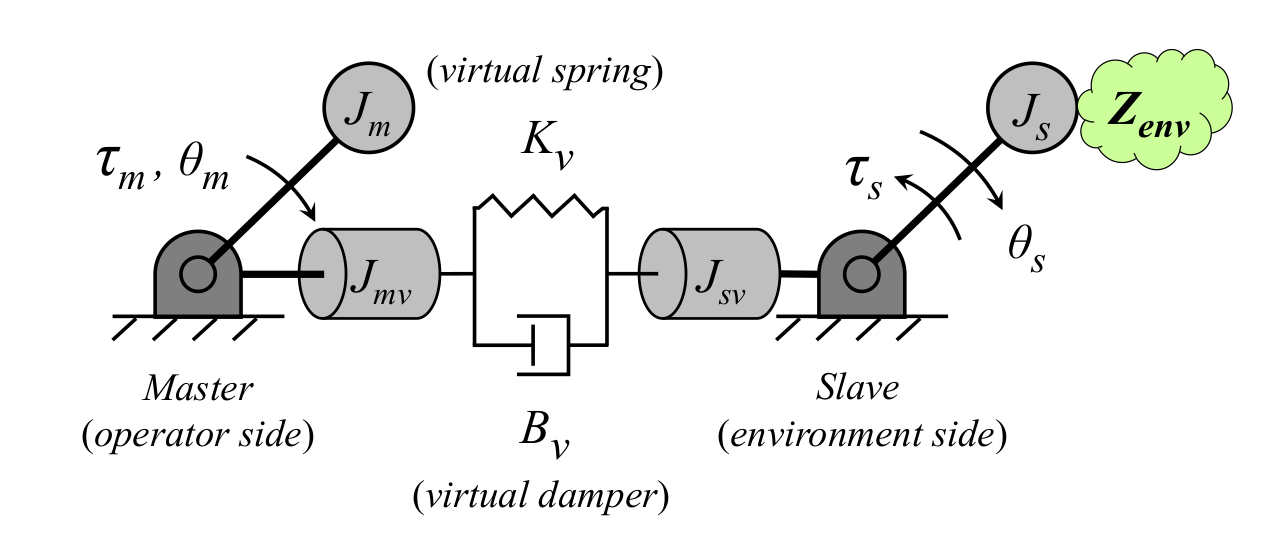
\includegraphics[width=0.8\linewidth]{../reportTeleop/Images/spring_damper_inertia_system}
	\end{figure}

%Position error based torque reflection to the operator at the master side.
	
	\begin{list}{$ \circ $}{}
		\item Real inertiae: $ J_{m}, J_{s} $
		\item Virtual inertiae: $ J_{mv}, J_{sv} $
		\item Virtual damper and spring: $ B_{v}, K_{v} $
	\end{list}

\end{frame}

\begin{frame}{Bilateral Control Scheme}

	\begin{figure}
	\centering
	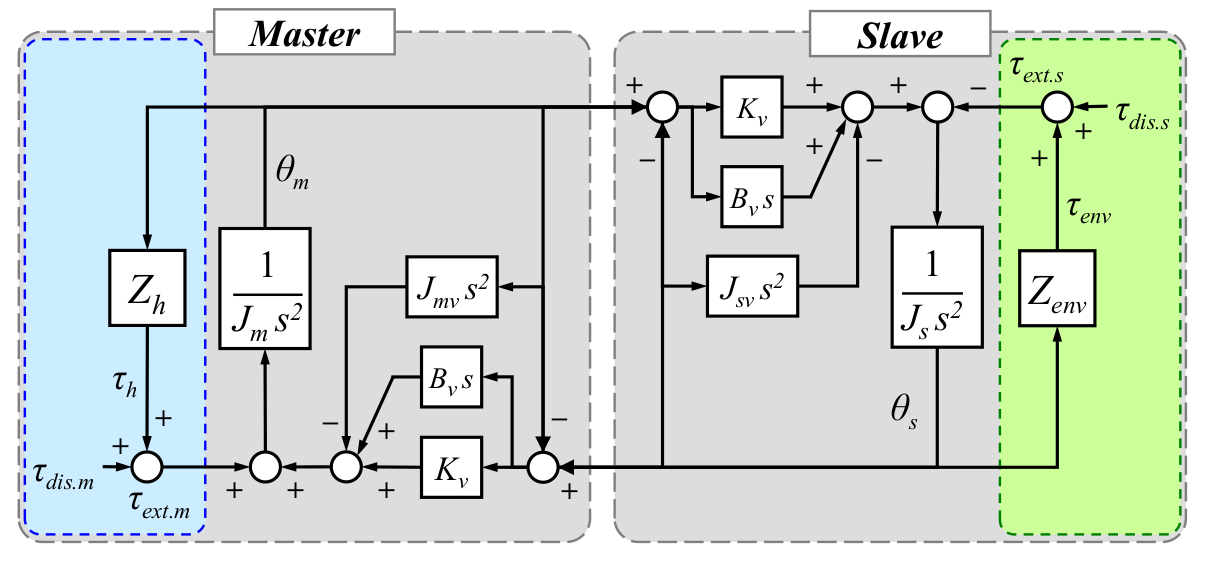
\includegraphics[width=0.8\linewidth]{../reportTeleop/Images/Block_diagram}
	\end{figure}

Dynamics equations of the system:
\begin{align*}
(J_m + J_{mv})\ddot{\theta}_m + B_v (\dot{\theta}_m - \dot{\theta}_s) + K_v(\theta_m - \theta_s) &= \tau_m \\
(J_s + J_{sv})\ddot{\theta}_s + B_v (\dot{\theta}_s - \dot{\theta}_m) + K_v(\theta_s - \theta_m) &= - \tau_s 
\end{align*}
	
\end{frame}


\begin{frame}[fragile]{Bilateral Controller}

%External torques as action and reaction torque of human and environment impedance, $ Z_{h} $ and $ Z_{env} $:
The virtual parameters are considered elements of the controller. Equations are rearranged:
\begin{align*}
	J_m s^2 \theta_m &= \tau_m - (B_v s + K_v) (\theta_m - \theta_s) - J_{mv} s^2 \theta_m \\
	J_s s^2 \theta_s &= - \tau_s - (B_v s + K_v) (\theta_s - \theta_m) - J_{sv} s^2 \theta_s
\end{align*}
where the external torques are action and reaction forces of the human and the environment.

System represented by:

\begin{equation*}
\begin{bmatrix}
\tau_m \\ \theta_s
\end{bmatrix} = 
\underbrace{\begin{bmatrix}
H_{11} & H_{12} \\
H_{21} & H_{22}
\end{bmatrix}}_{\text{\textit{Hybrid matrix}}}
\begin{bmatrix}
\theta_m \\ - \tau_s
\end{bmatrix}
\label{hybrid_matrix}
\end{equation*}

\end{frame}

\begin{frame}[fragile]{Bilateral Controller}

Hybrid parameters $ H_{ij} $:
\begin{align*}
	H_{11} &= \frac{1}{Z_s}[Z_m Z_s - (B_v s + K_v)^2] \\
	H_{12} &= -\frac{1}{Z_s}[B_v s + K_v] \\
	H_{21} &= \frac{1}{Z_s}[B_v s + K_v] \\
	H_{22} &= \frac{1}{Z_s} 
\end{align*}
where:
\begin{align*}
	Z_m &= (J_m + J_{mv}) s^2 + B_v s + K_v \\
	Z_s &= (J_s + J_{sv}) s^2 + B_v s + K_v
\end{align*}

\end{frame}

\begin{frame}{Bilateral Controller}

\textit{Condition of transparency}: trasmitted impedance $ Z_{t} $ transferred to the operator should be equal to environment impedance $ Z_{env} $:
\begin{equation*}
	\frac{\tau_m}{\theta_m} = Z_t = Z_{env} = \frac{\tau_s}{\theta_s}
\end{equation*}
Relationship between $ Z_{t} $ and $ Z_{env} $:
\begin{equation*}
	Z_t = \big(\dfrac{-H_{12} H_{21}}{1 + H_{22} Z_{env}}\big)Z_{env} + H_{11}
\end{equation*}

%Hybrid parameters for the perfect transparency condition, derived as:
%\begin{equation*}
%	\begin{bmatrix}
%	\tau_m \\ \theta_s
%	\end{bmatrix} = 
%	\begin{bmatrix}
%	0 & -1 \\ 1 & 0
%	\end{bmatrix}
%	\begin{bmatrix}
%	\theta_m \\ -\tau_s
%	\end{bmatrix}
%\end{equation*}

\end{frame}

%\section{System Analysis}

\section{Vibration Suppression Design}

\begin{frame}{Parameters Selection and Design}

Assume system disturbed by environment vibration noise.\\
\bigskip
Inspect $ H_{22} $ for the relationship of position response $ \theta_s $ and external torque input $ \tau_{ext} $:
\begin{equation*}
	\dfrac{\theta_s}{\tau_{ext}} = \dfrac{1}{(J_s + J_{sv}) s^2 + B_v s + K_v}
	\label{H_22}
\end{equation*}\\
\bigskip
Virtual parameters $ J_{v}, B_{v} $ and $ K_{v} $ determined from the characteristic equation:
\begin{equation*}
	s^{2} + (g_{1} + g_{2})s + (g_{1} \cdot g_{2}) = 0
\end{equation*}
%established from two poles $ g_{1} $ and $ g_{2} $, representing the desired cut-off frequencies of the system for disturbance suppression.
where the poles $ g_1 $ and $ g_2 $ represent the desired cut-off frequencies.

\end{frame}

\begin{frame}{Parameters Selection and Design}
	
Spring stiffness $ K_{v} $ influences the transparency.\\
\bigskip
It regulates the \textit{compliance} of the system, achieving \textbf{rigid coupling} (high spring stiffness) or \textbf{spring coupling} (low spring stiffness).\\
\bigskip
\pause
{\centering
\Ovalbox{We want to chose $ K_v $ beforehand!}\par}
\pause

\bigskip
Virtual parameters $ B_{v} $ and $J_{v} $ computed according to $ K_{v} $:
\begin{equation*}
	B_v = \left(\frac{g_1 + g_2}{g_1 \cdot g_2}\right) K_v
\end{equation*}
and
\begin{equation*}
	J_{sv} = \left(\frac{1}{g_1 \cdot g_2}\right) K_v - J_s
\end{equation*}

\end{frame}	


% \begin{frame}{}
% \end{frame}	

\section{Simulations}

\begin{frame}{Simulation conditions}
	Simulation are done in ideal condition:
	\begin{itemize}
		\item the communication between master and slave have no critical aspects;
		\item instantaneous and loss-less signal transfer.
	\end{itemize}
	
	We will compare two different settings:
	\begin{table}[H]
		\centering
		\begin{tabular}{c c c c}
			\toprule
			Behaviour & $K_{v}$ & $B_{v}$ &  $J_{v}$\\
			\midrule 
			\midrule 
			Virtual compliance& $20.0 \ \frac{\text{N m}}{\text{rad}} $ & $4.4\cdot 10^{-1} \ \frac{\text{N m}}{\text{rad/s}}$ & $3\cdot 10^{-4} \ \text{kg m\textsuperscript{2}}$\\
			Rigid coupling & $10^{2} \ \frac{\text{N m}}{\text{rad}} $ & $1.5\cdot 10^{-1} \ \frac{\text{N m}}{\text{rad/s}}$ & $ 0 \ \text{kg m\textsuperscript{2}} $\\
			\bottomrule
		\end{tabular}
		\caption{Sets of chosen virtual parameters.}
		\label{virtParams}
	\end{table}

\end{frame}

\subsection*{Vibration Suppression Performances}
\begin{frame}{Disturbance response}
	
  \begin{equation*}
    \dfrac{\theta_s}{\tau_{ext}} = \dfrac{1}{(J_s + J_{sv}) s^2 + B_v s + K_v}
  \end{equation*}\\
  \begin{figure}
  	\centering
  	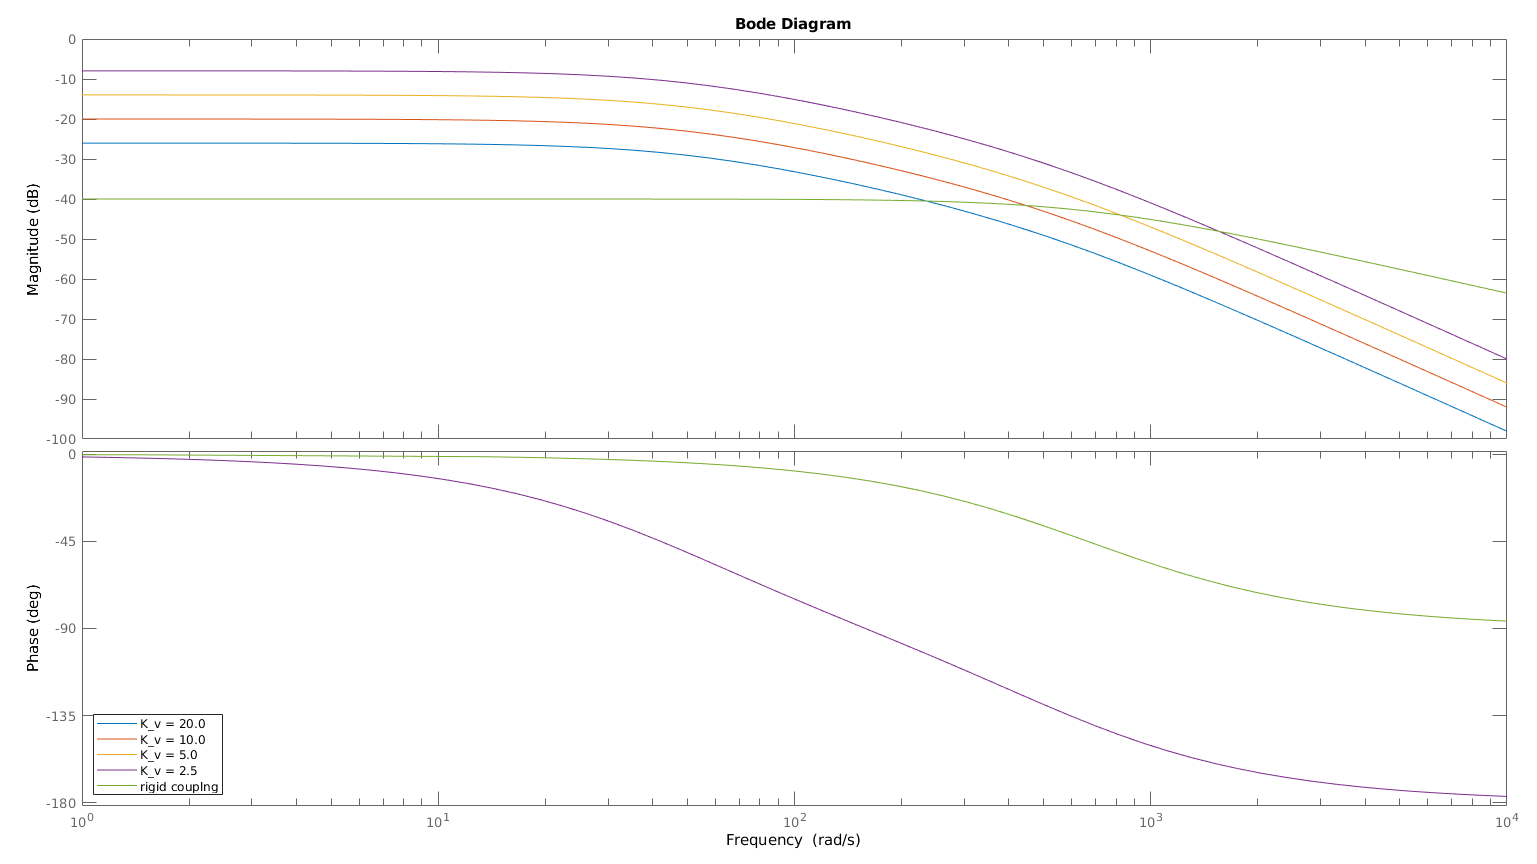
\includegraphics[width=1\linewidth]{../reportTeleop/Images/bodo}
%  	\caption{}
%  	\label{fig:bodeplot2}
  \end{figure}
  
%  \begin{center}
%    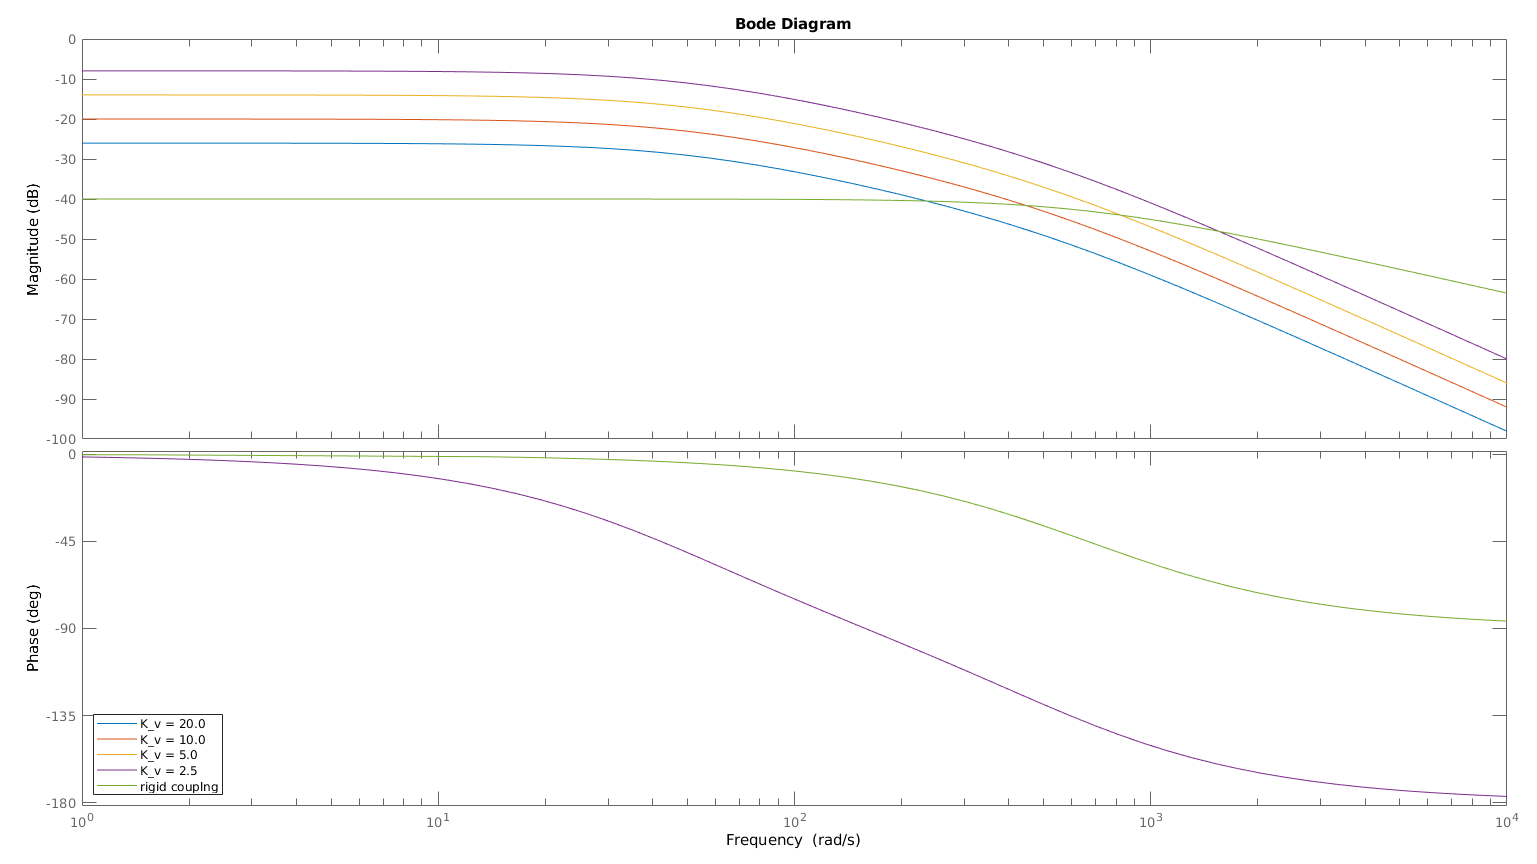
\includegraphics[width=\textwidth, height=0.45\textwidth]{../reportTeleop/Images/bodeplot2}\\
%    \bigskip
%    \begin{tabular}{c|c c c c c c}
%       & Set I & Set II & Set III & Set IV & Rigid coupling & \\
%      \midrule 
%	    $K_{v}$ & $ 20.0 $ & $ 10.0 $ & $ 5.0 $ & $ 2.5 $ & $ 100.0 $ & $ \frac{\text{N} \cdot \text{m}}{\text{rad}} $ \\
%    \end{tabular}
%  \end{center}

\end{frame}

\begin{frame}{Vibration suppression}
  \begin{center}
    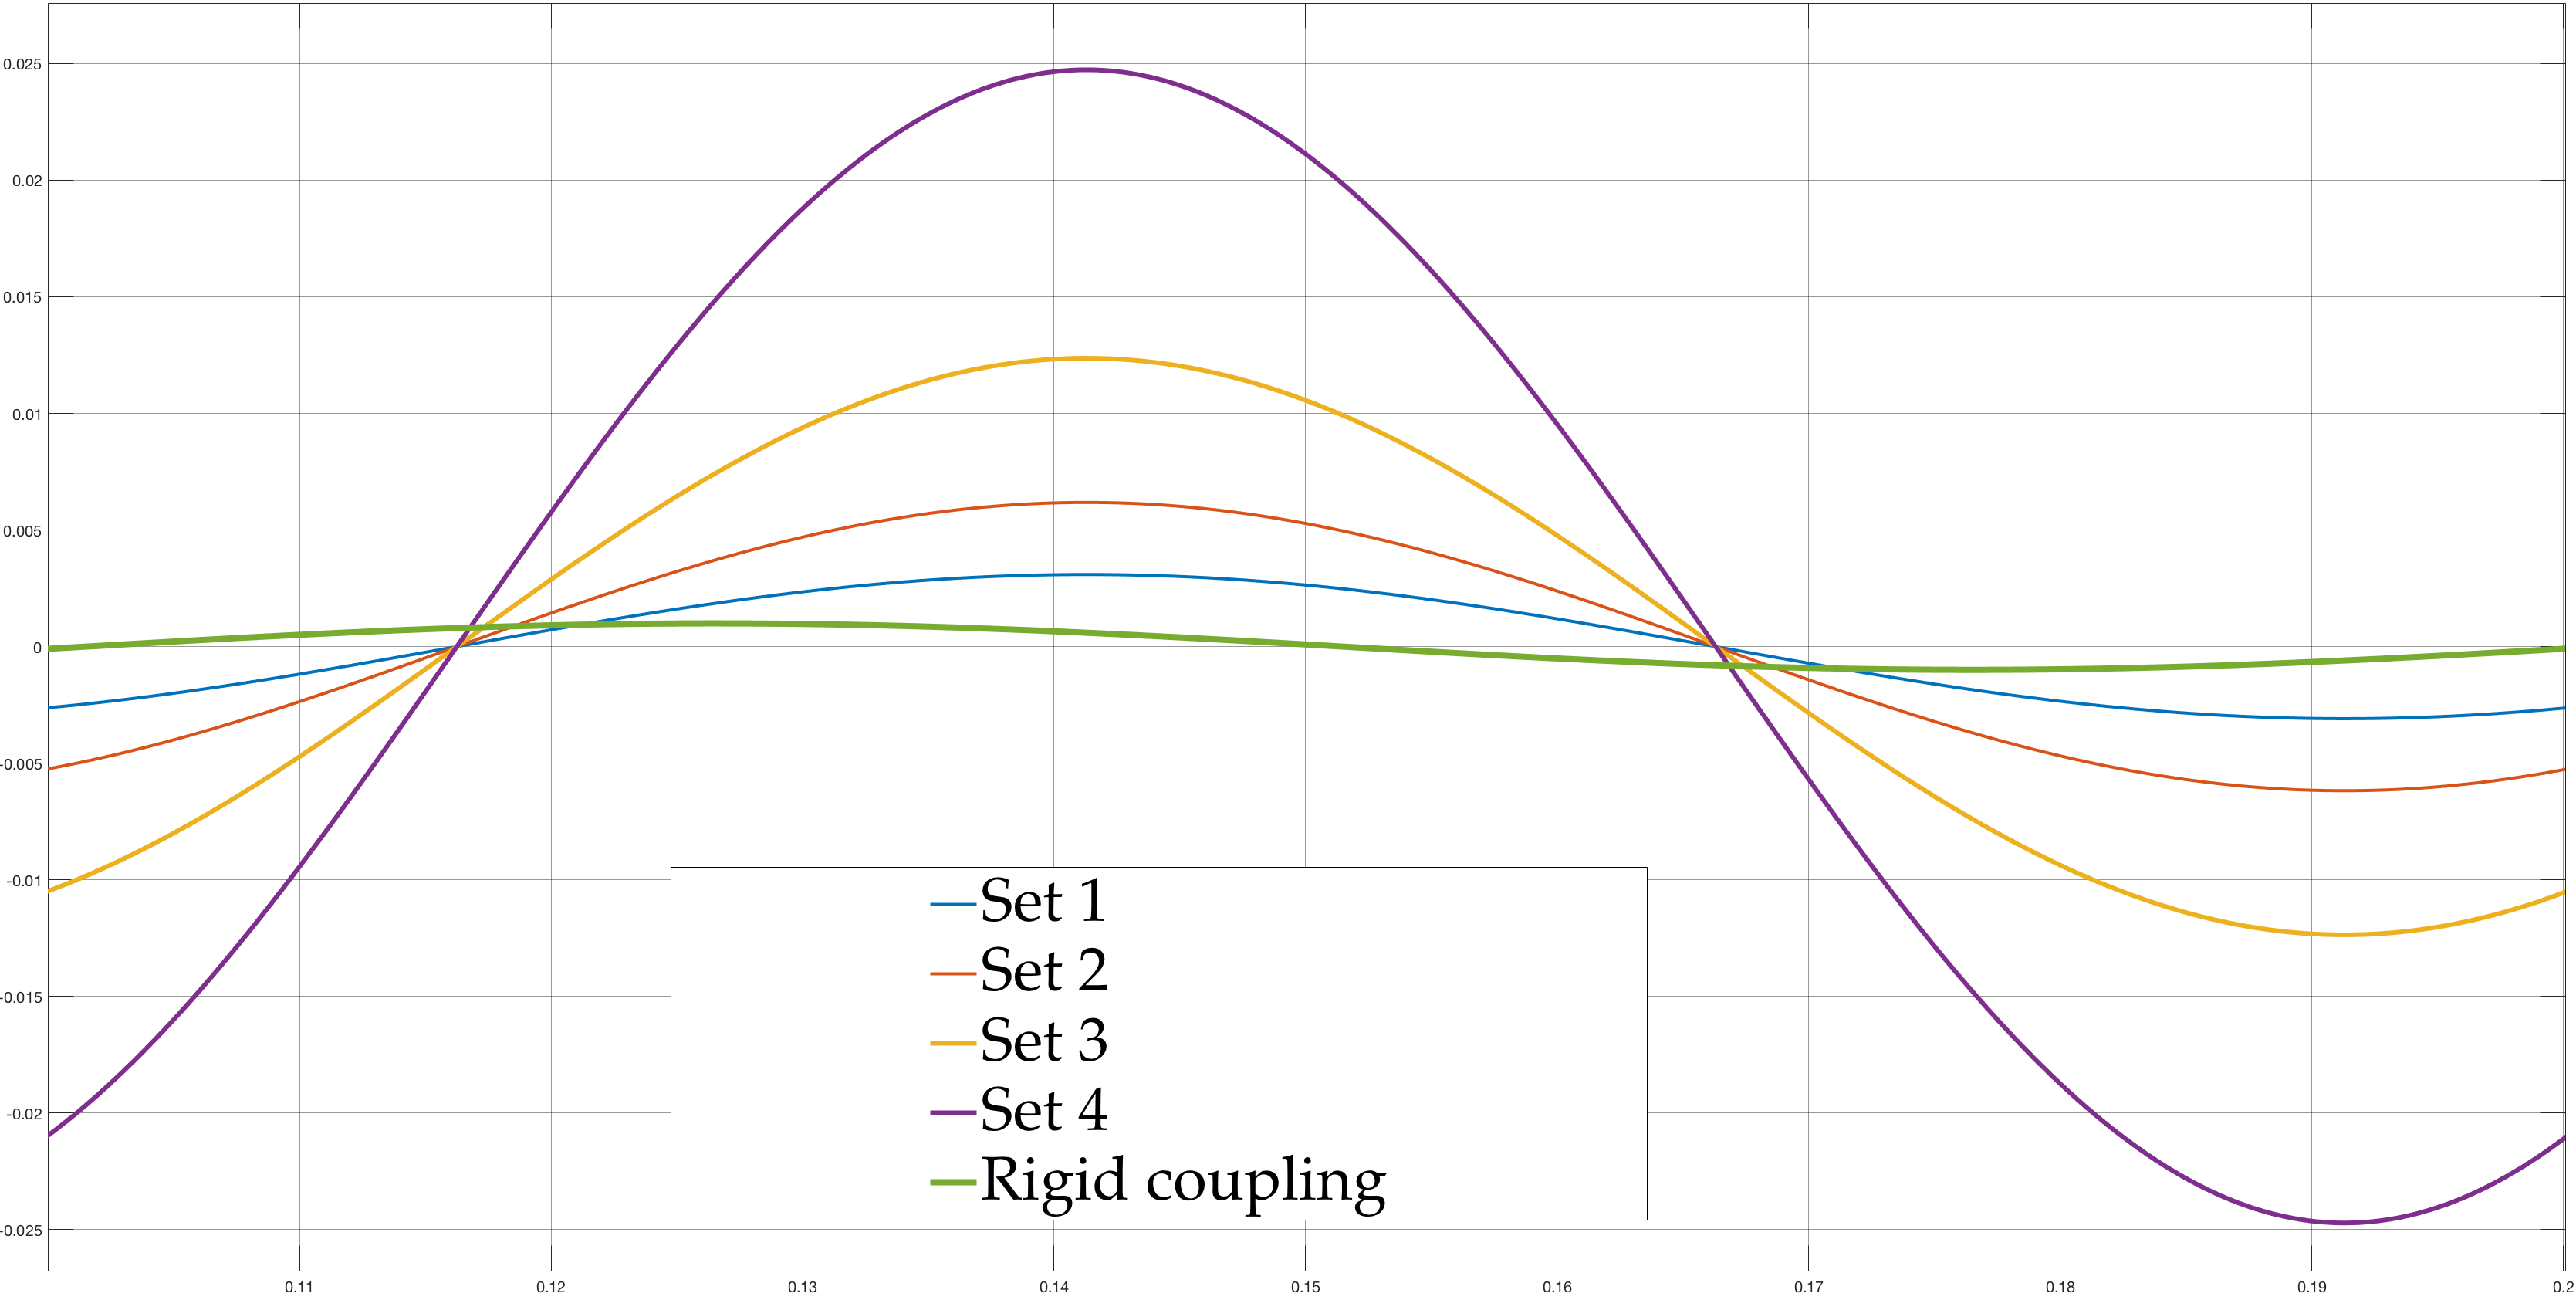
\includegraphics[width=\textwidth, height=0.21\textwidth]{../reportTeleop/Images/vibr10Htz}\\
    \smallskip
    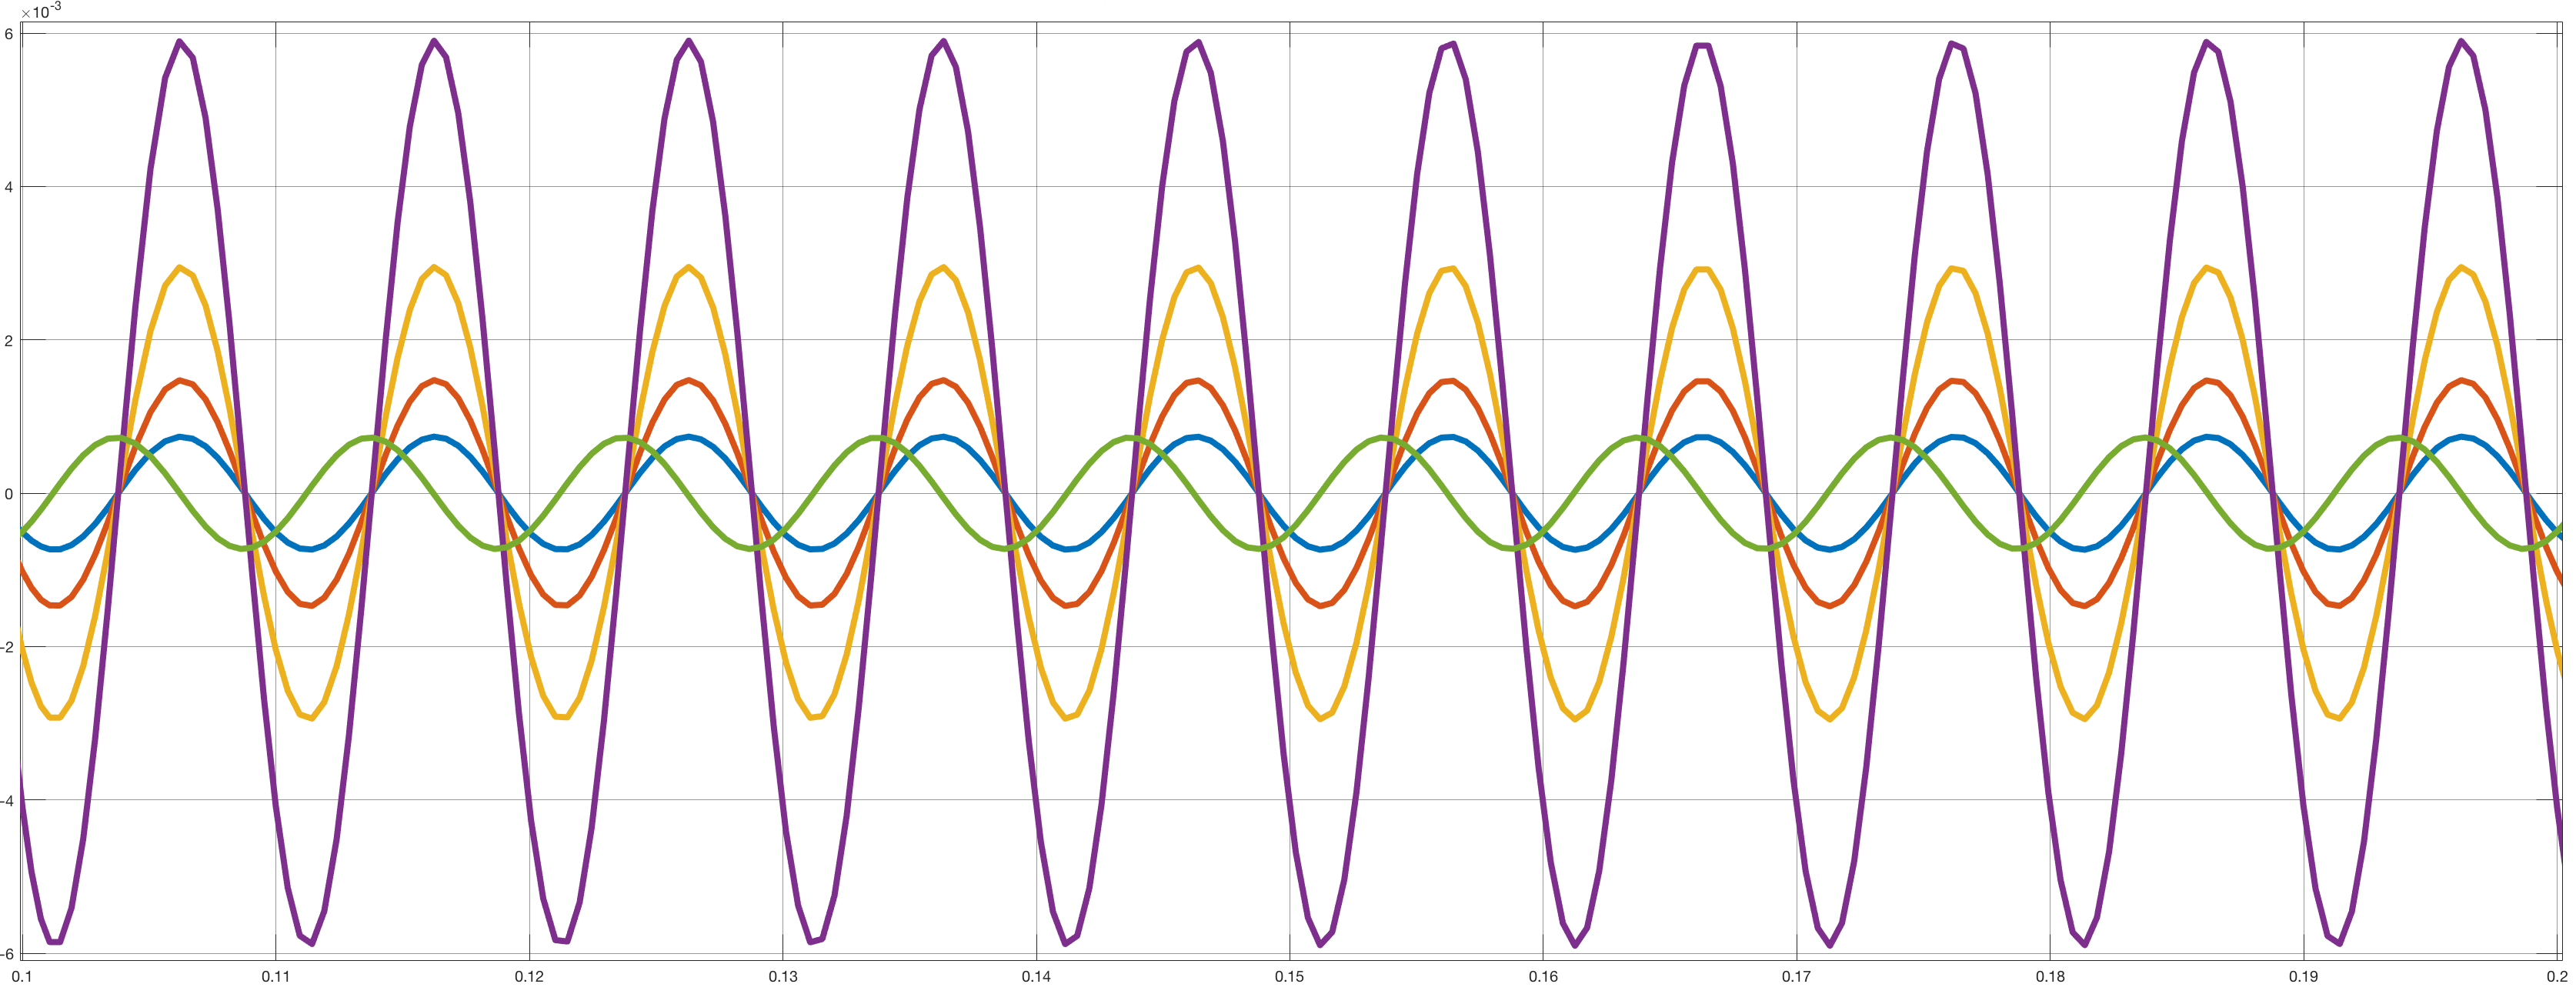
\includegraphics[width=\textwidth, height=0.21\textwidth]{../reportTeleop/Images/vibr100Htz}\\
    \smallskip
    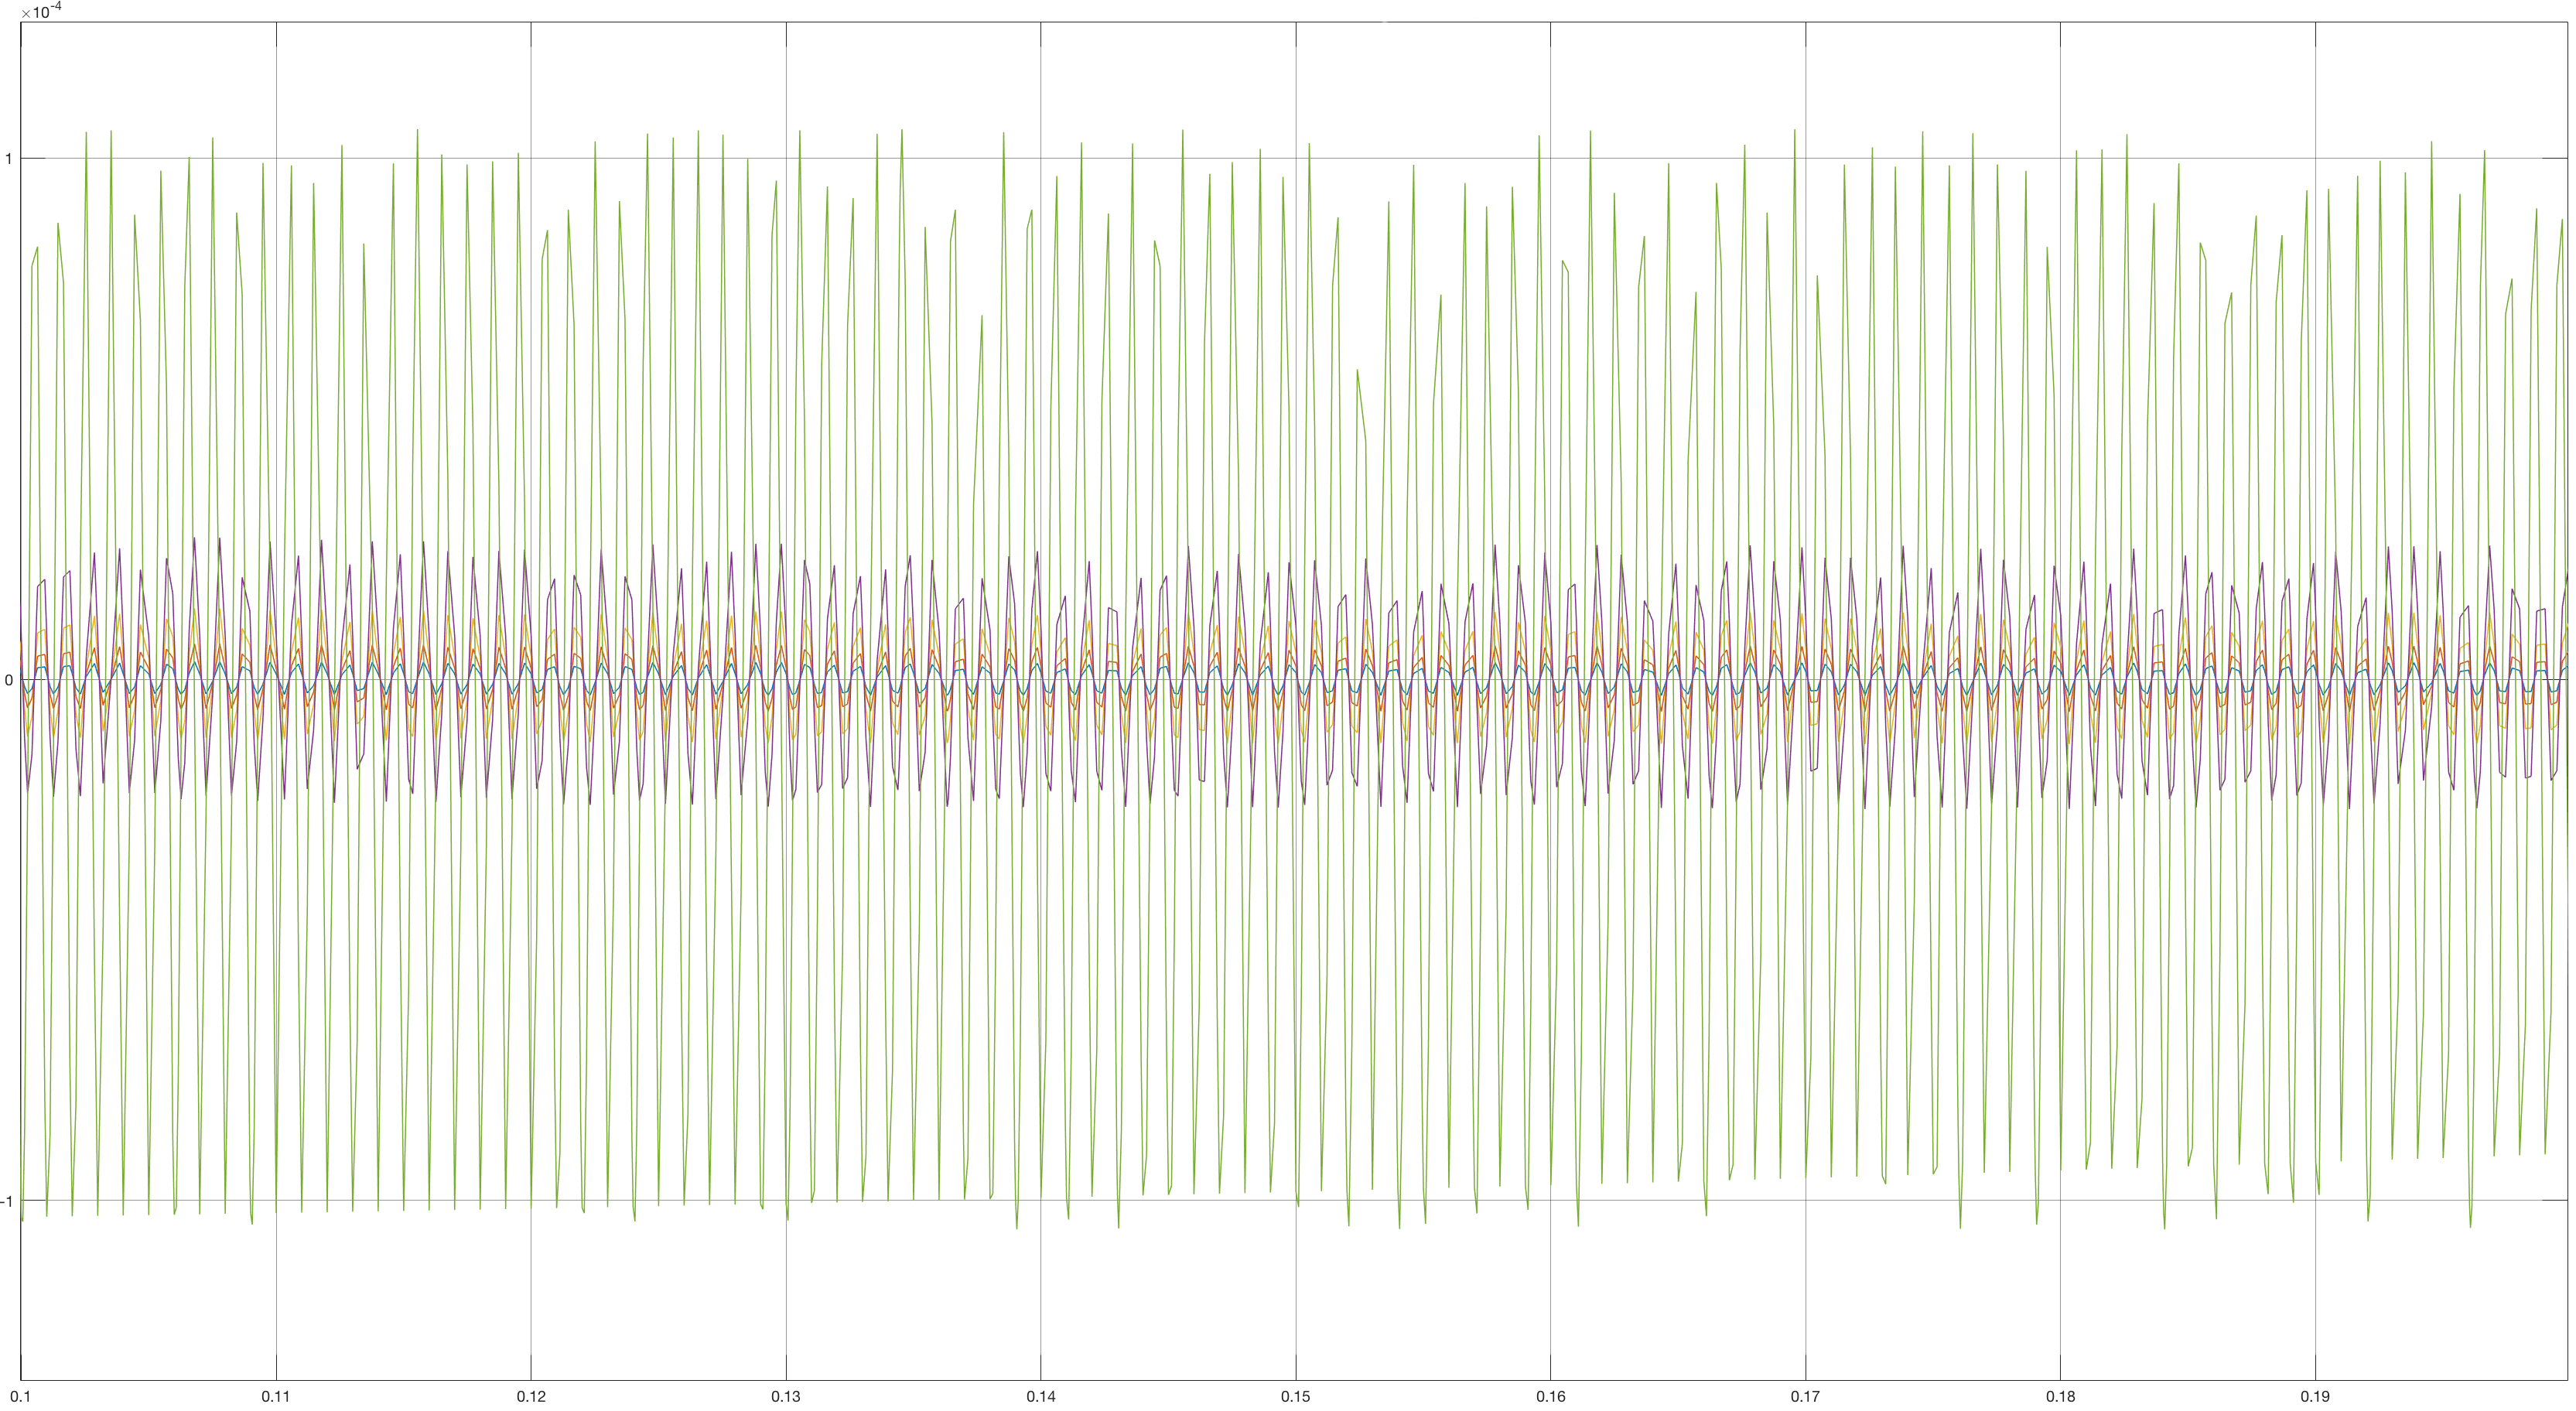
\includegraphics[width=\textwidth, height=0.21\textwidth]{../reportTeleop/Images/vibr1000Htz}\\
    \begin{tabular}{c  c | c | c }
      \textbf{ Noise frequency :} & 10 Hz & $10^2$ Hz & $10^3$ Hz \\
    \end{tabular}
 \end{center}
\end{frame}

\subsection*{Task execution performances}

%\begin{frame}{Task execution:  Free Motion}
%  \begin{columns}
%    \column{.75\textwidth}
%    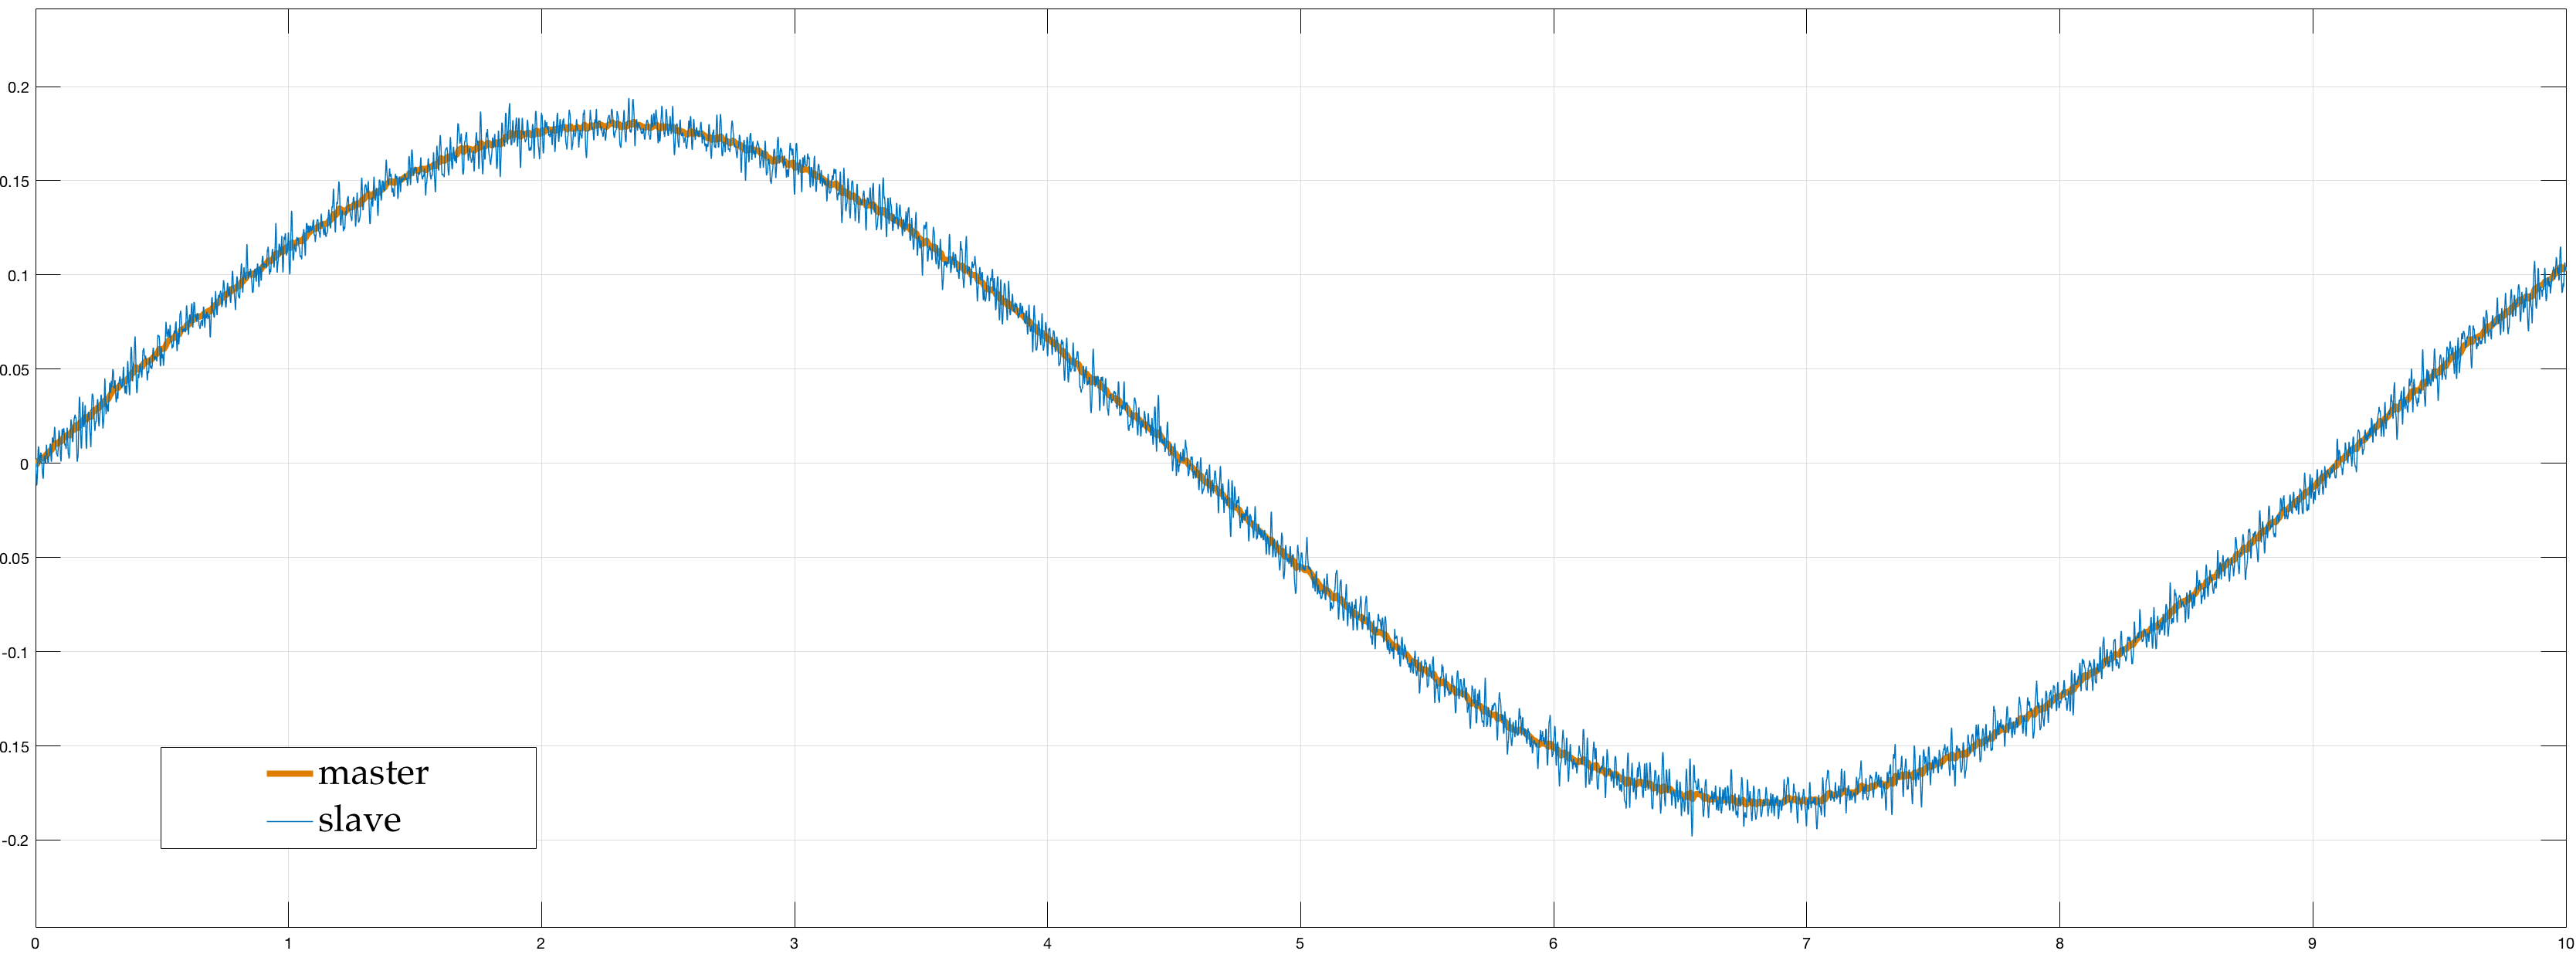
\includegraphics[width=\textwidth,
%    height=0.45\textwidth]{../reportTeleop/Images/rCoupFreeTot50htznoise}\\
%    \smallskip
%    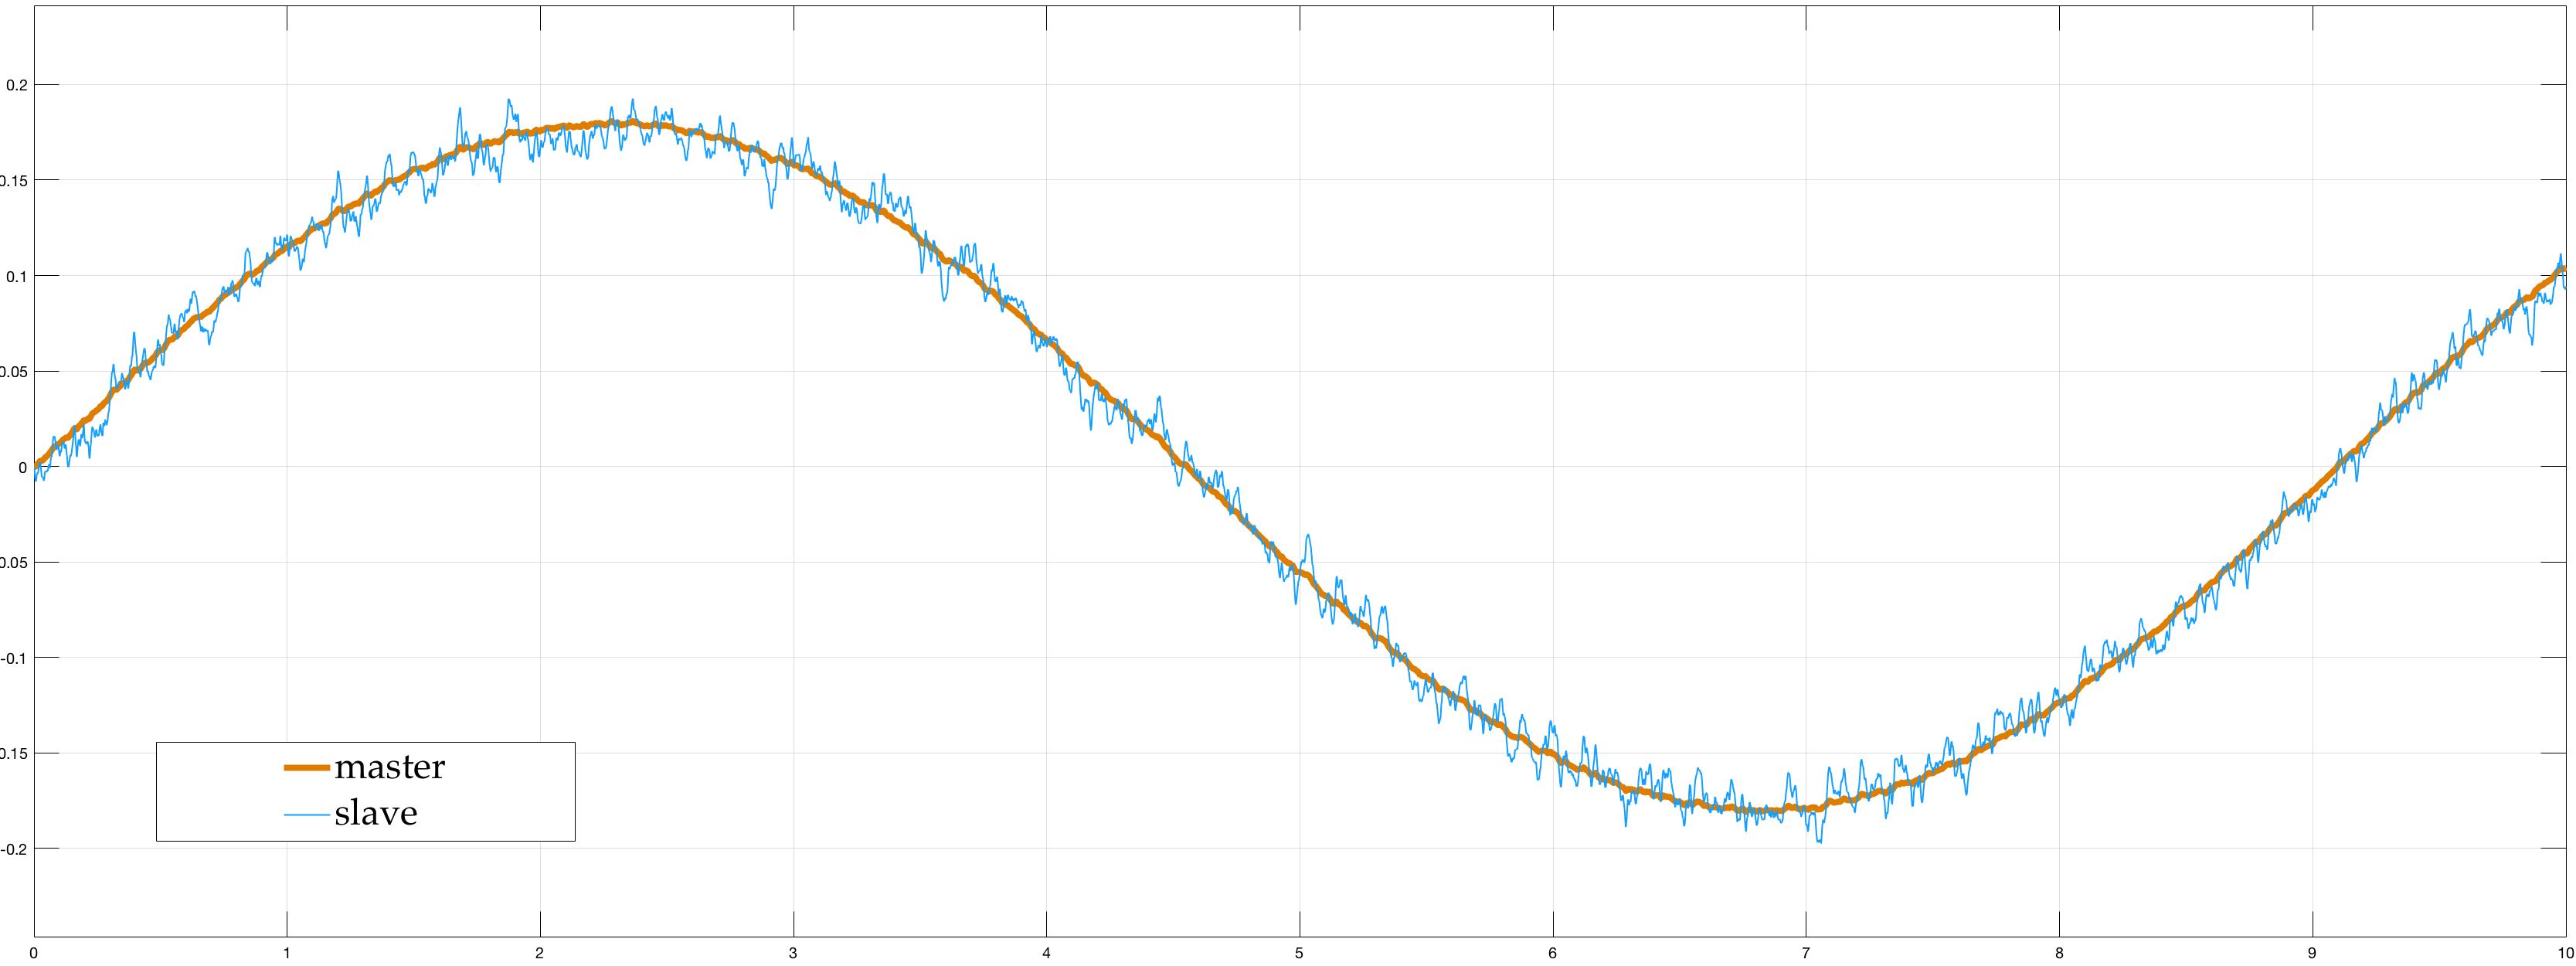
\includegraphics[width=\textwidth,
%    height=0.45\textwidth]{../reportTeleop/Images/set20freeTot50Htznoise}
%    \column{.30\textwidth}
%
%    \textbf{Rigid coupling}:\\
%    \begin{itemize}
%    \item{High transparency}
%    \item{A lot of vibrations}
%    \end{itemize}
%    \smallskip
%
%    \textbf{Virtual compliance}:\\
%    \begin{itemize}
%    \item{ A bit less \textsl{responsive}}
%    \item{\textsl{Smoother} (vibrations damped)}
%    \end{itemize}
%  \end{columns}
%\end{frame}

\begin{frame}{Free Motion: High frequency noise}
\smallskip
\begin{columns}
	\column{.20\textwidth}
	\color{Orange}\textbf{Rigid coupling:}\\
	\bigskip
	\bigskip
	\bigskip
	\color{black}\textbf{High frequency:} 50 Hz\\
	\bigskip
	\bigskip
	\bigskip
	\color{LightBlue}\textbf{Virtual compliance:}\\
	
	\column{.85\textwidth}
	
	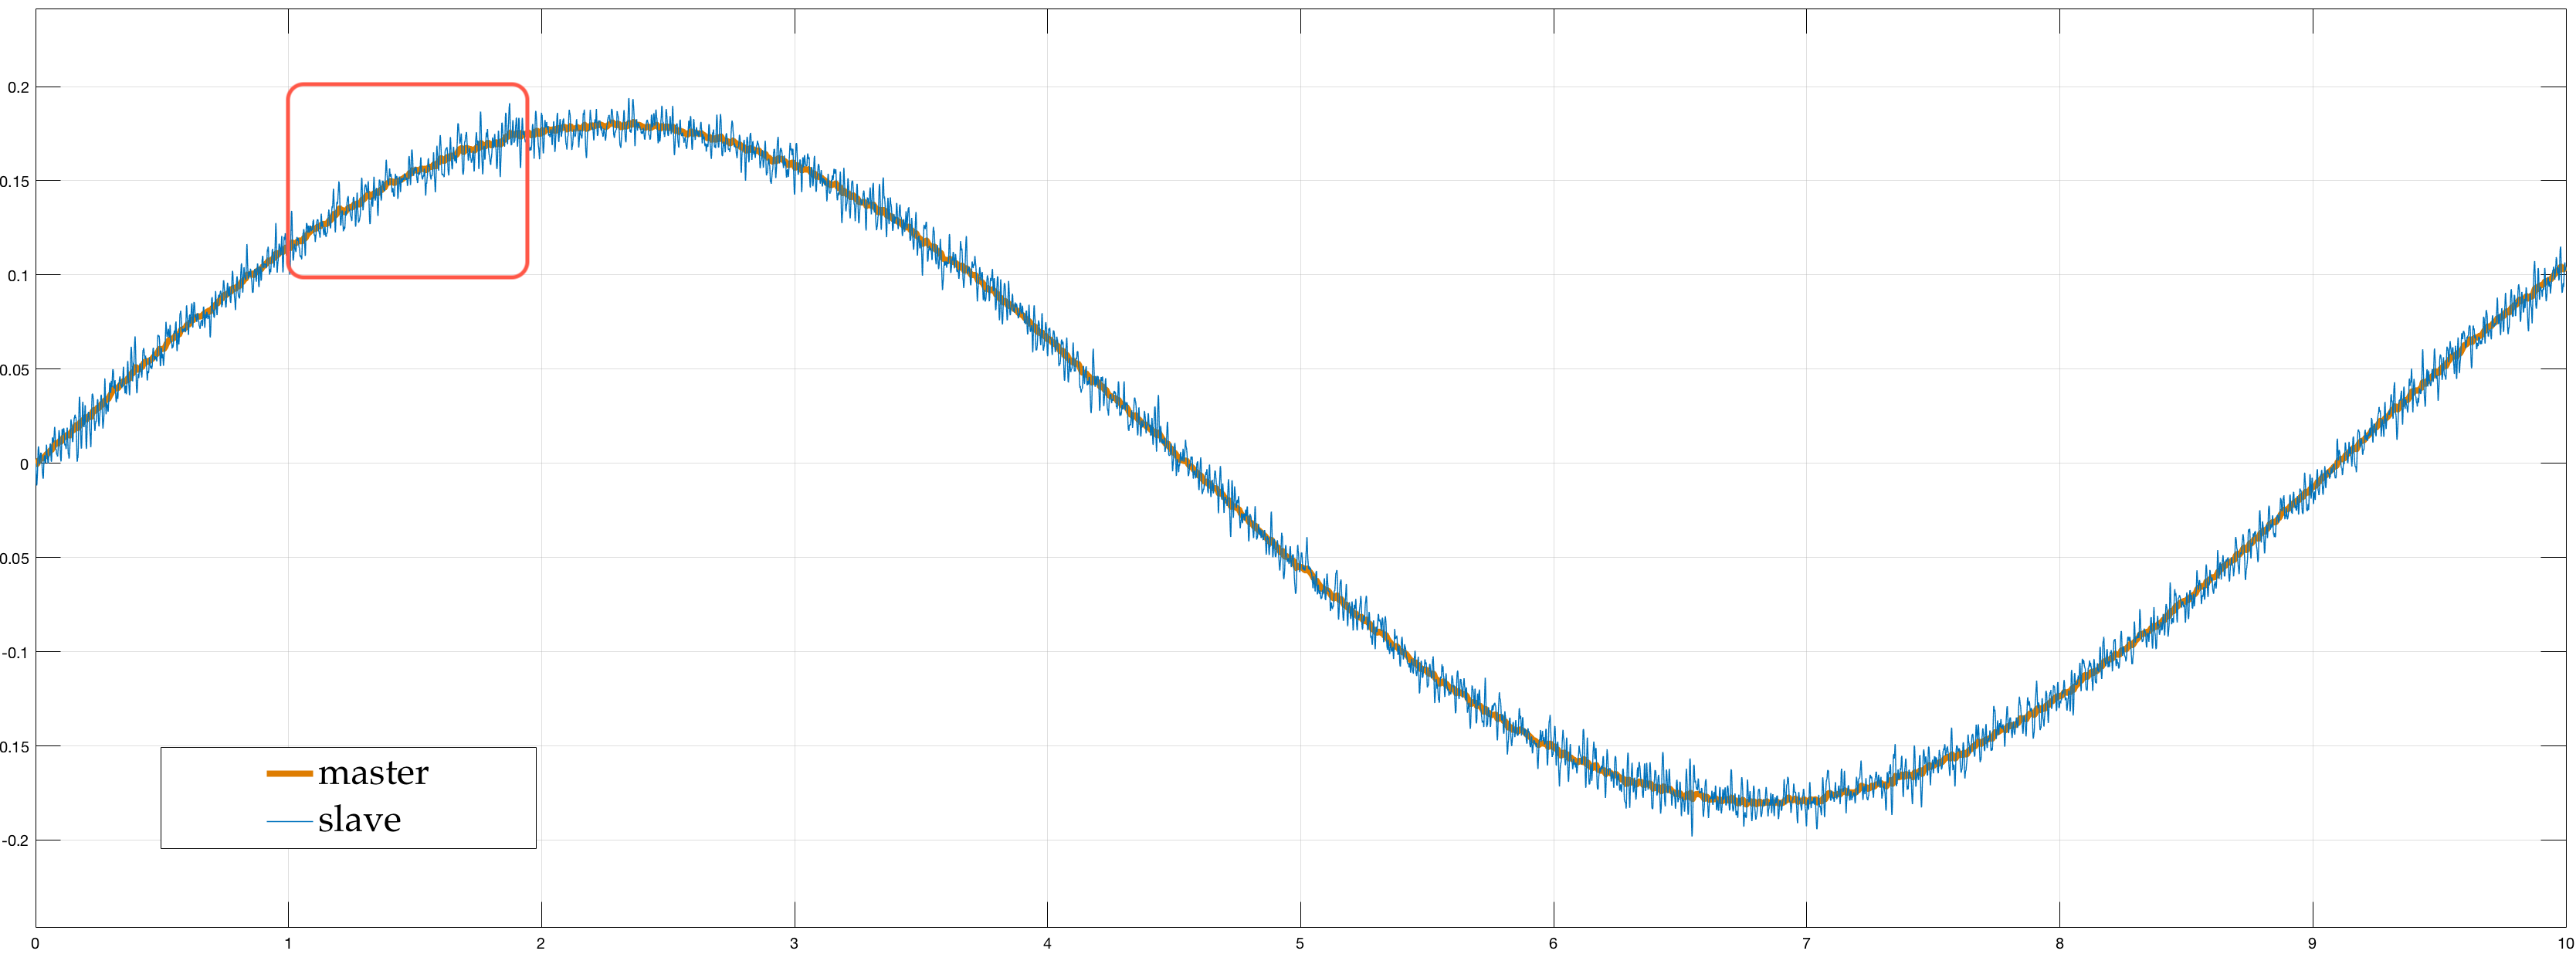
\includegraphics[width=\textwidth,
	height=0.45\textwidth]{../reportTeleop/Images/rCoupFreeTot50htznoiseRect}\\
	\smallskip
	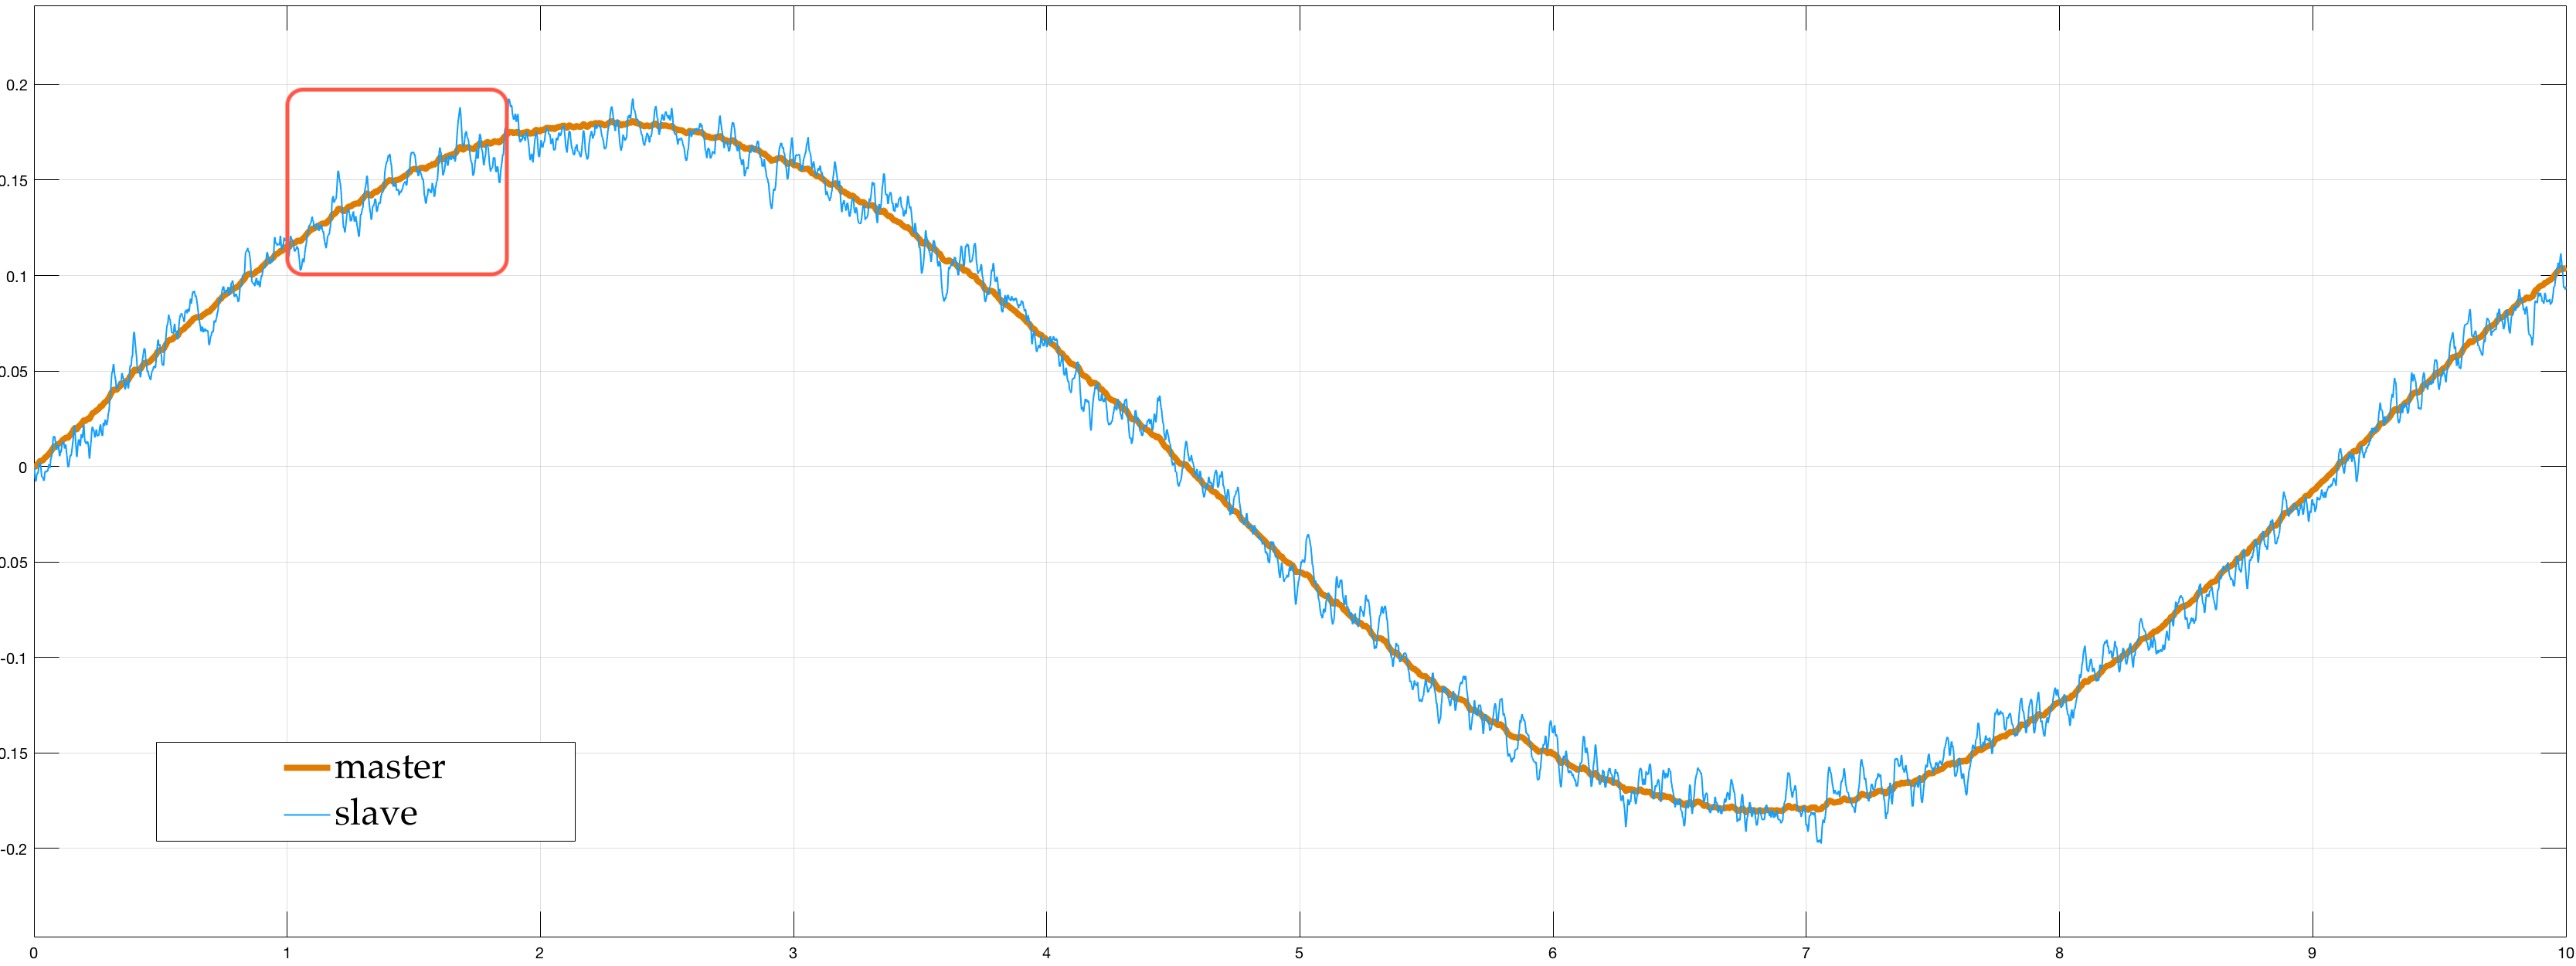
\includegraphics[width=\textwidth,
	height=0.45\textwidth]{../reportTeleop/Images/set20freeTot50HtznoiseRect}
\end{columns}

\end{frame}

\begin{frame}{Free Motion: High frequency noise}
\smallskip
\begin{columns}
\column{.20\textwidth}
\color{Orange}\textbf{Rigid coupling:}\\
\bigskip
\bigskip
\bigskip
\color{black}\textbf{High frequency:} 50 Hz\\
\bigskip
\bigskip
\bigskip
\color{LightBlue}\textbf{Virtual compliance:}\\

\column{.85\textwidth}

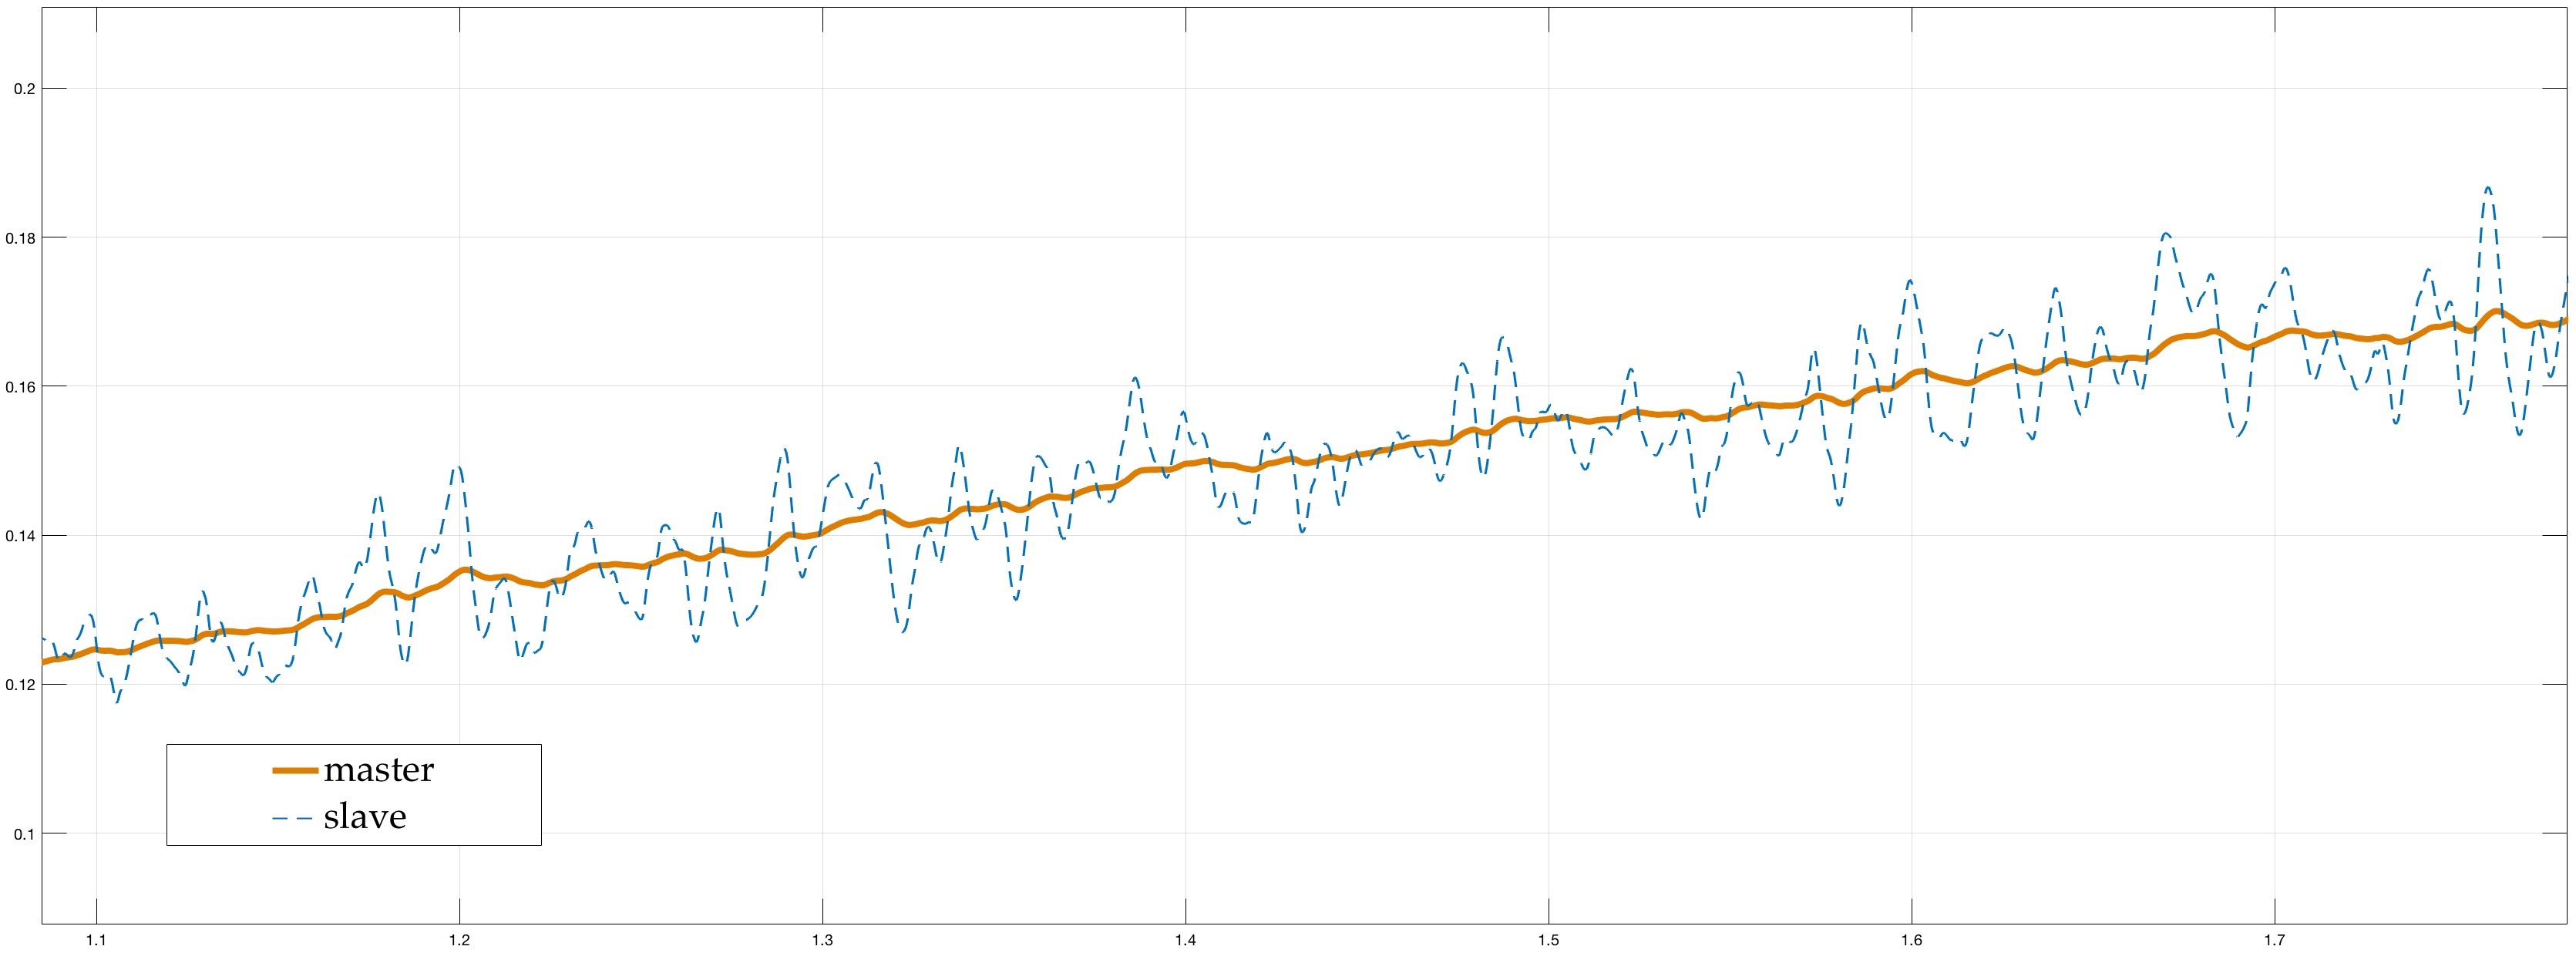
\includegraphics[width=\textwidth,
height=0.45\textwidth]{../reportTeleop/Images/rCoupFree50htznoise}\\
\smallskip
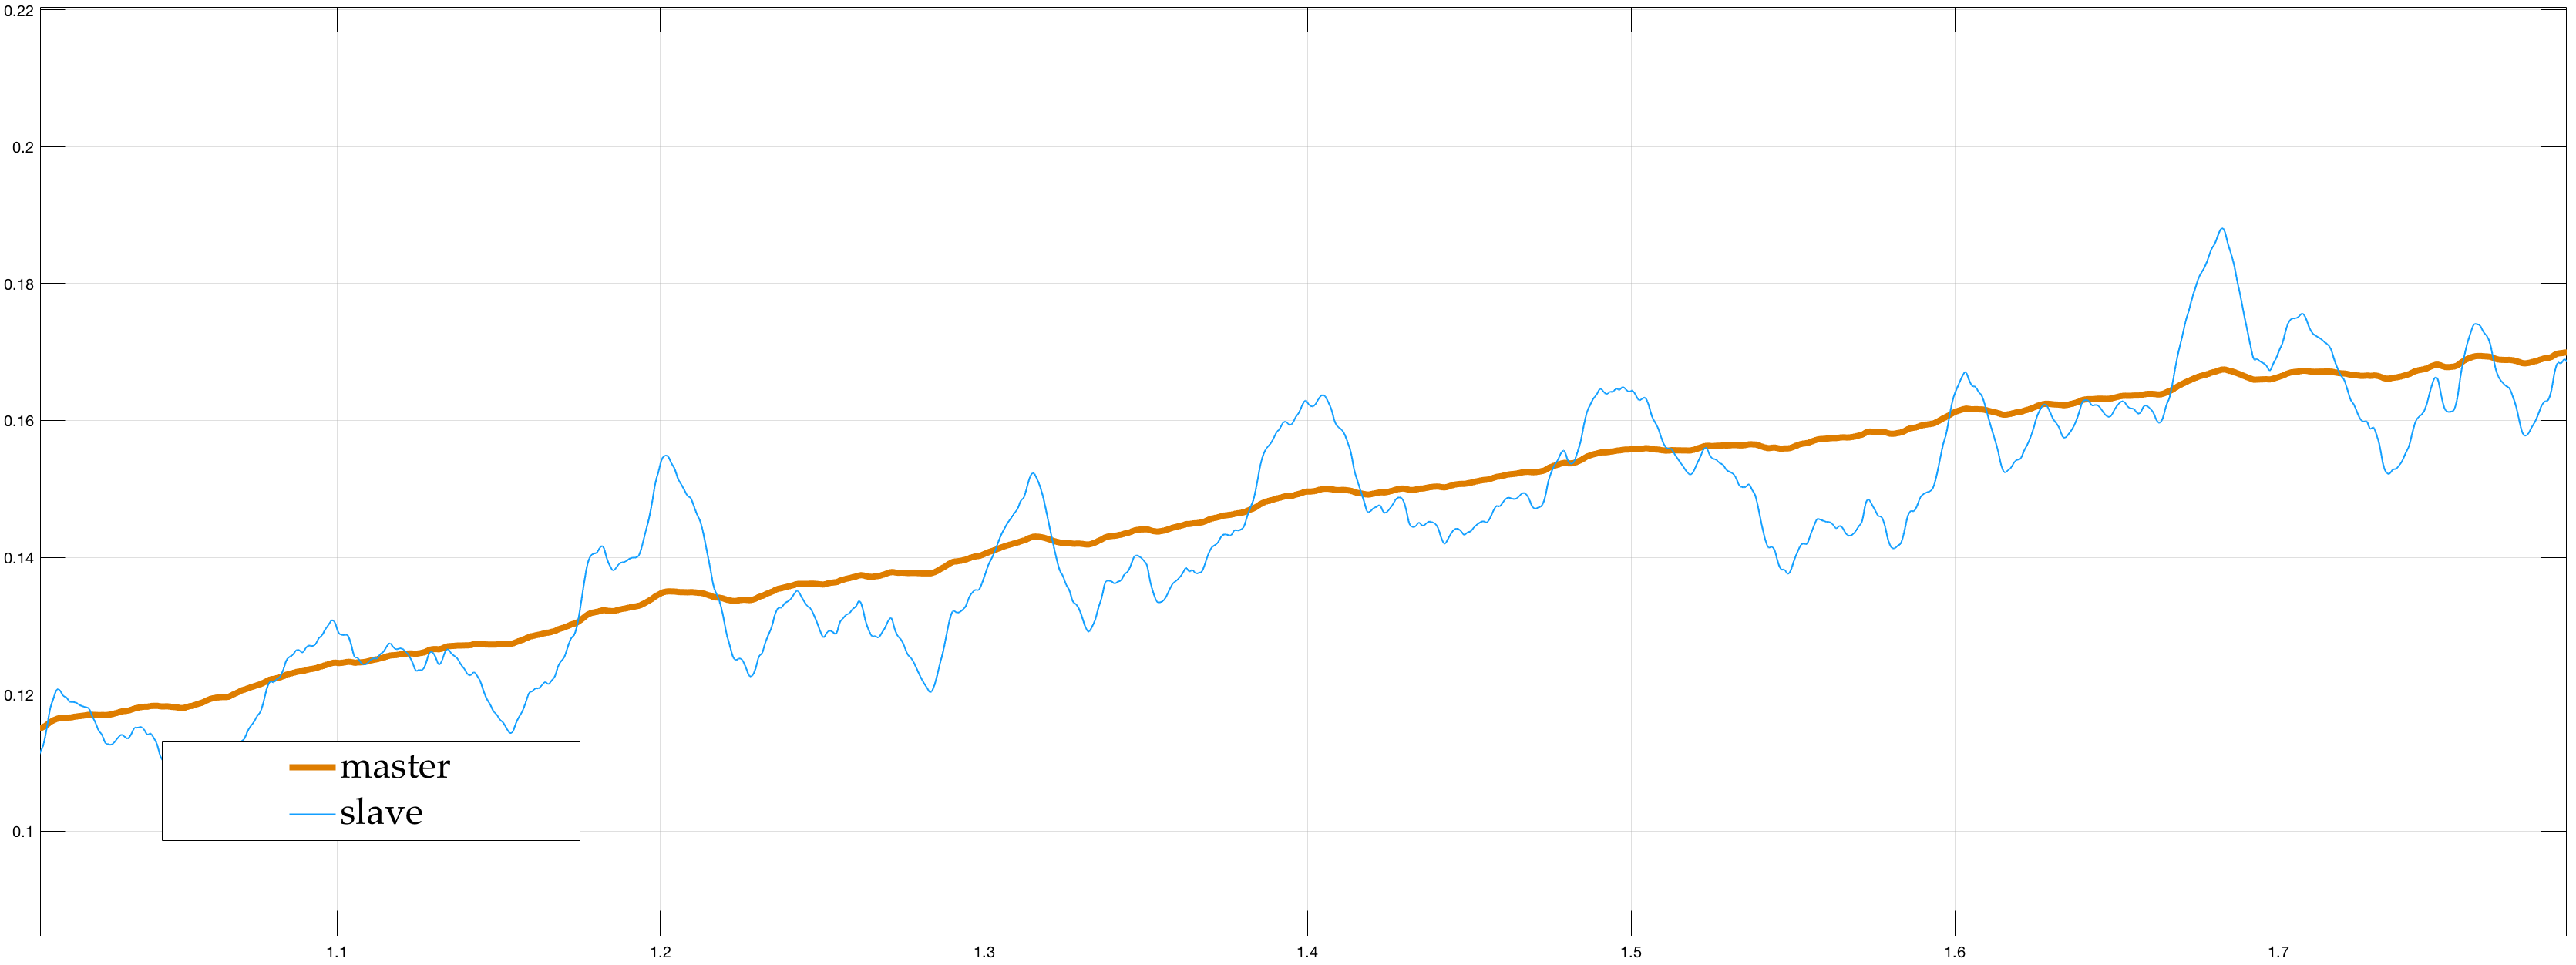
\includegraphics[width=\textwidth,
height=0.45\textwidth]{../reportTeleop/Images/set20freePart50Htznoise}
\end{columns}


\end{frame}

\begin{frame}{Free Motion: Low frequency noise 20 Hz}
\smallskip
\begin{columns}
	\column{.20\textwidth}
	\color{Orange}\textbf{Rigid coupling:}\\
	\bigskip
	\bigskip
	\bigskip
	\color{black}\textbf{Low frequency:} 20 Hz\\
	\bigskip
	\bigskip
	\bigskip
	\color{LightBlue}\textbf{Virtual compliance:}\\
	
	\column{.85\textwidth}
	
	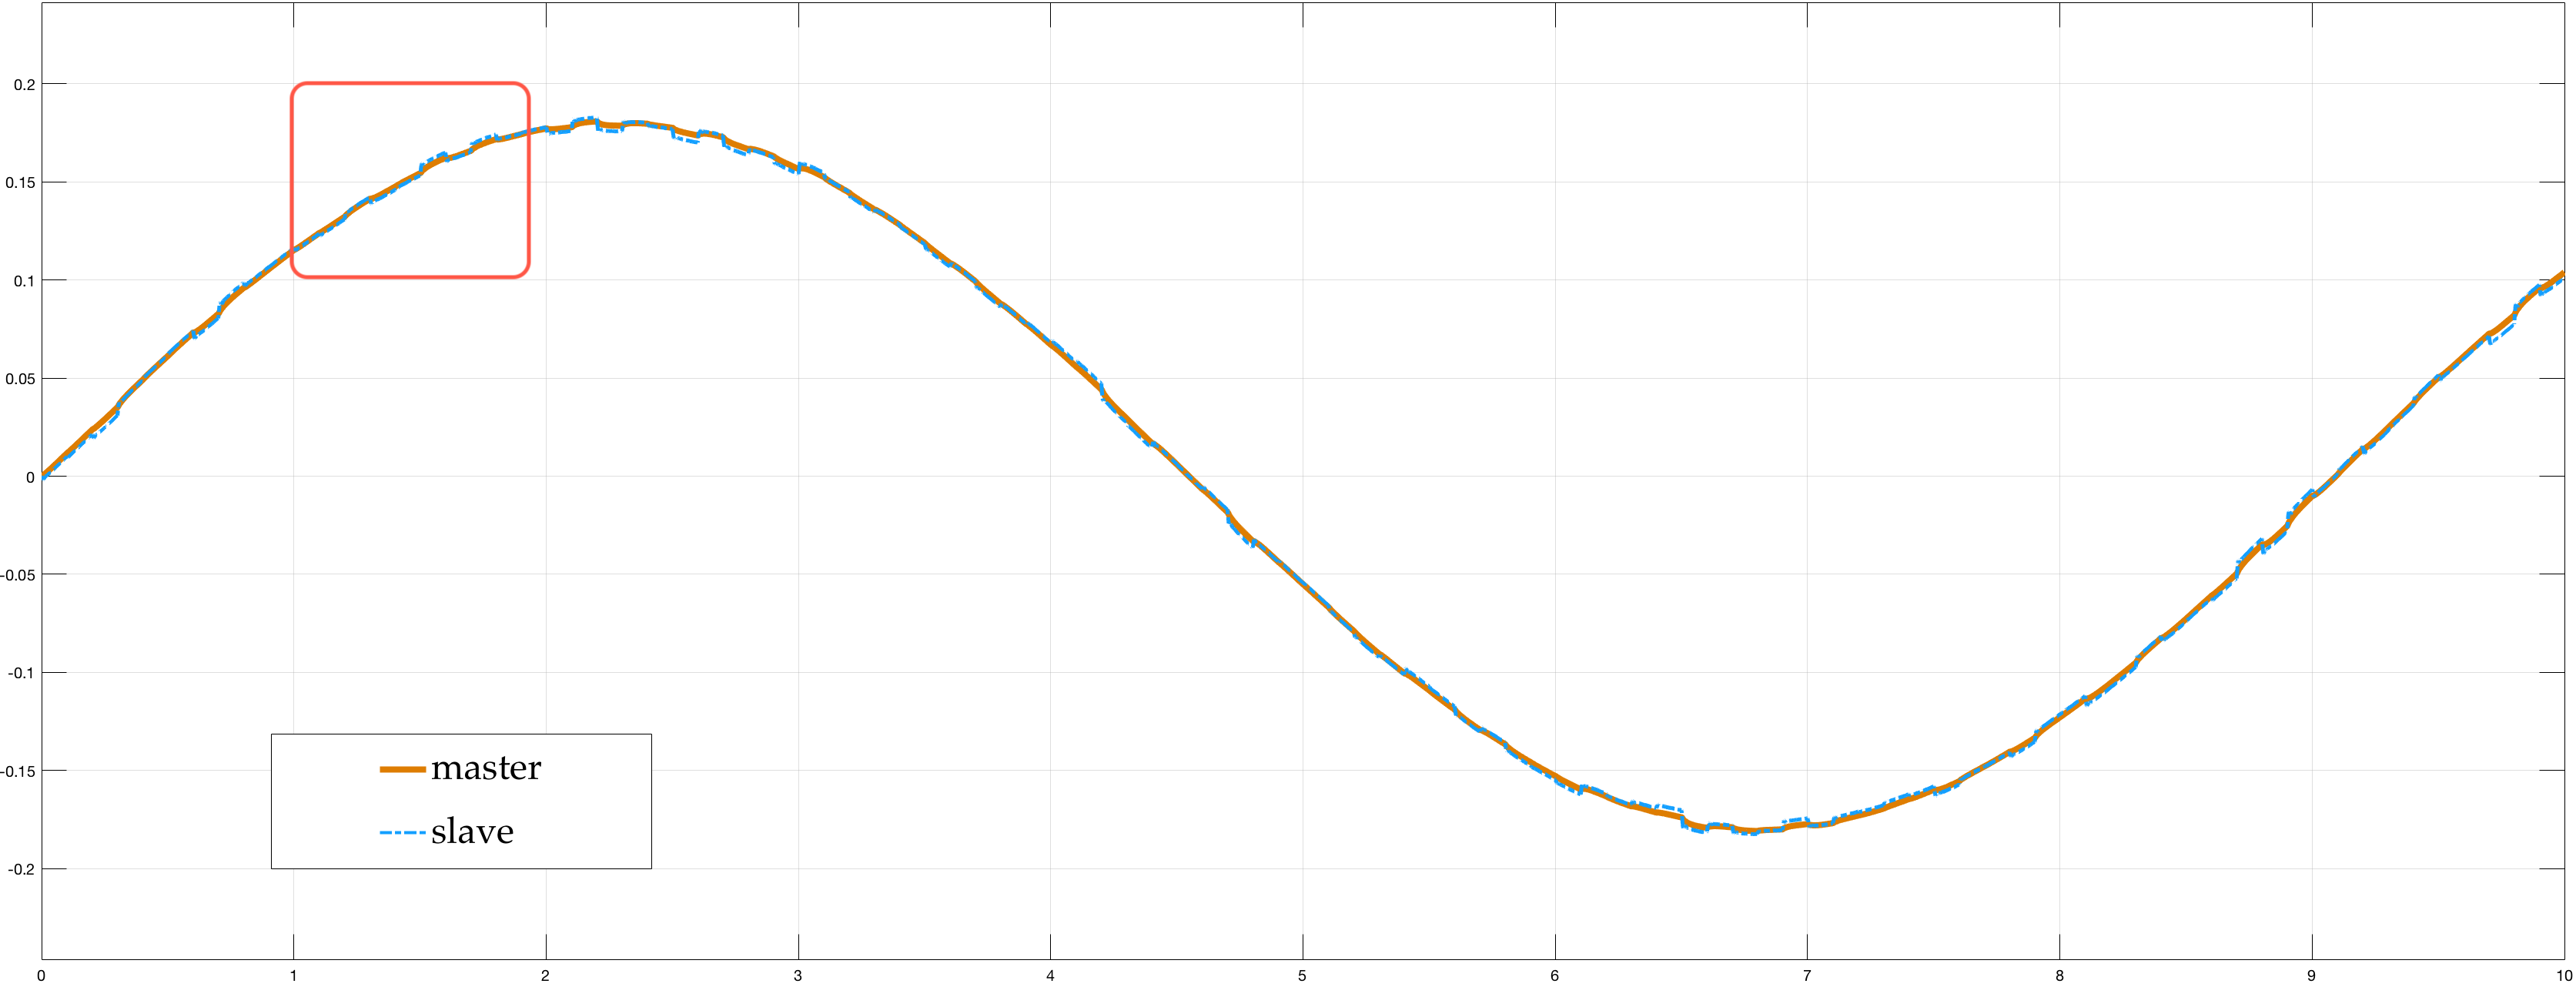
\includegraphics[width=\textwidth,
	height=0.45\textwidth]{../reportTeleop/Images/freerigidTot20HtznoiseRect}\\
	\smallskip
	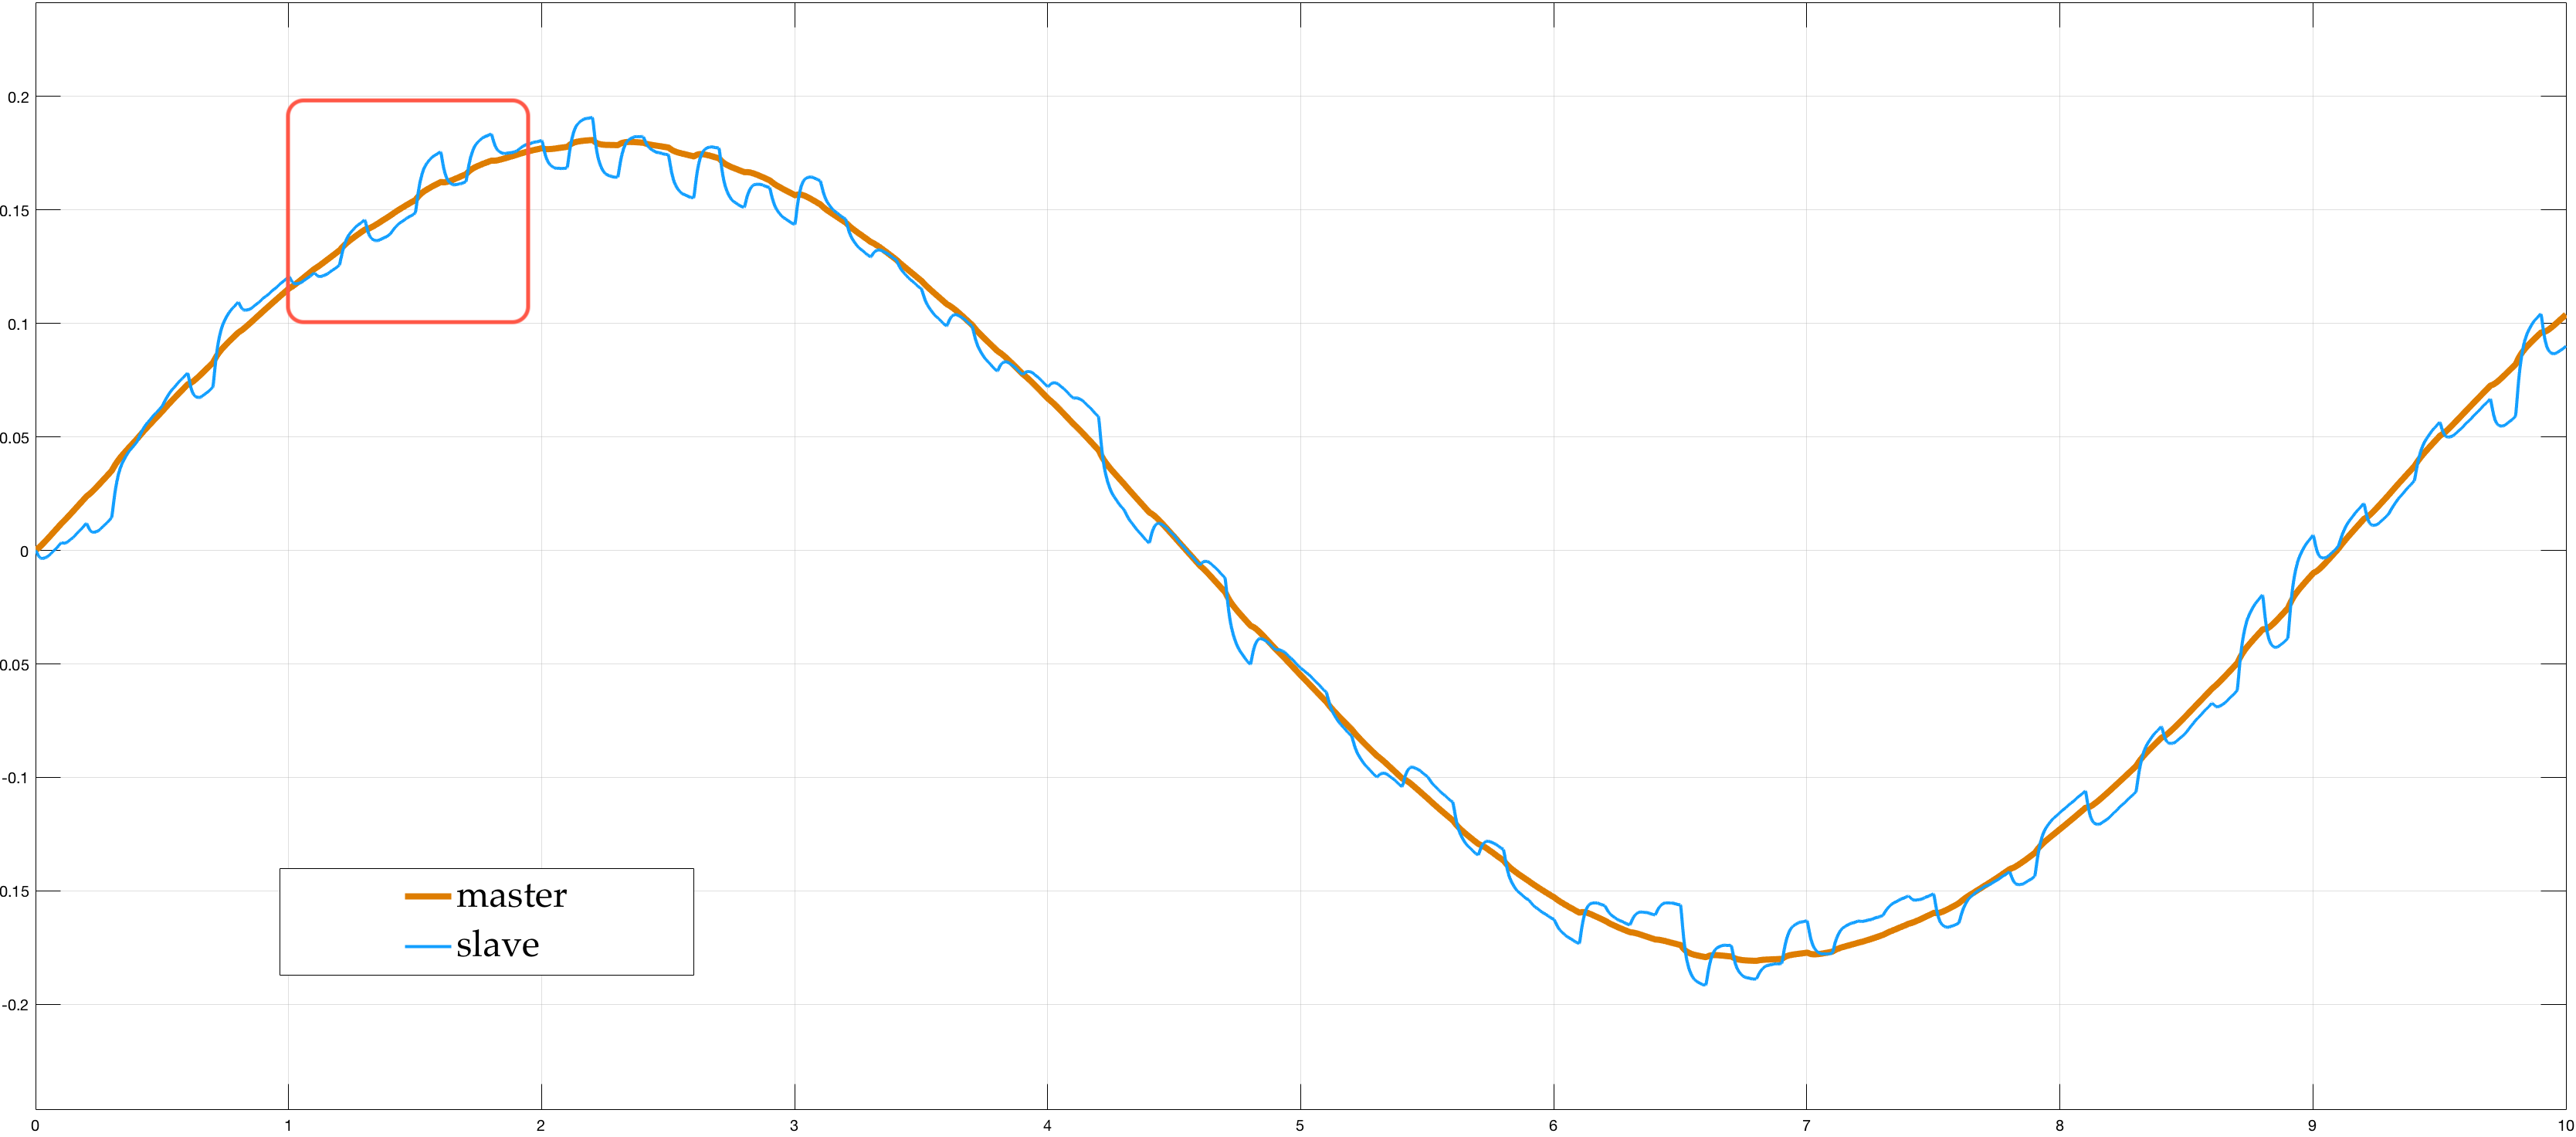
\includegraphics[width=\textwidth,
	height=0.45\textwidth]{../reportTeleop/Images/freeSet20Tot20HtznoiseRect}
\end{columns}

\end{frame}

\begin{frame}{Free Motion: Low frequency noise 20 Hz}
\smallskip
\begin{columns}
\column{.20\textwidth}
\color{Orange}\textbf{Rigid coupling:}\\
\bigskip
\bigskip
\bigskip
\color{black}\textbf{Low frequency:} 20 Hz\\
\bigskip
\bigskip
\bigskip
\color{LightBlue}\textbf{Virtual compliance:}\\

\column{.85\textwidth}

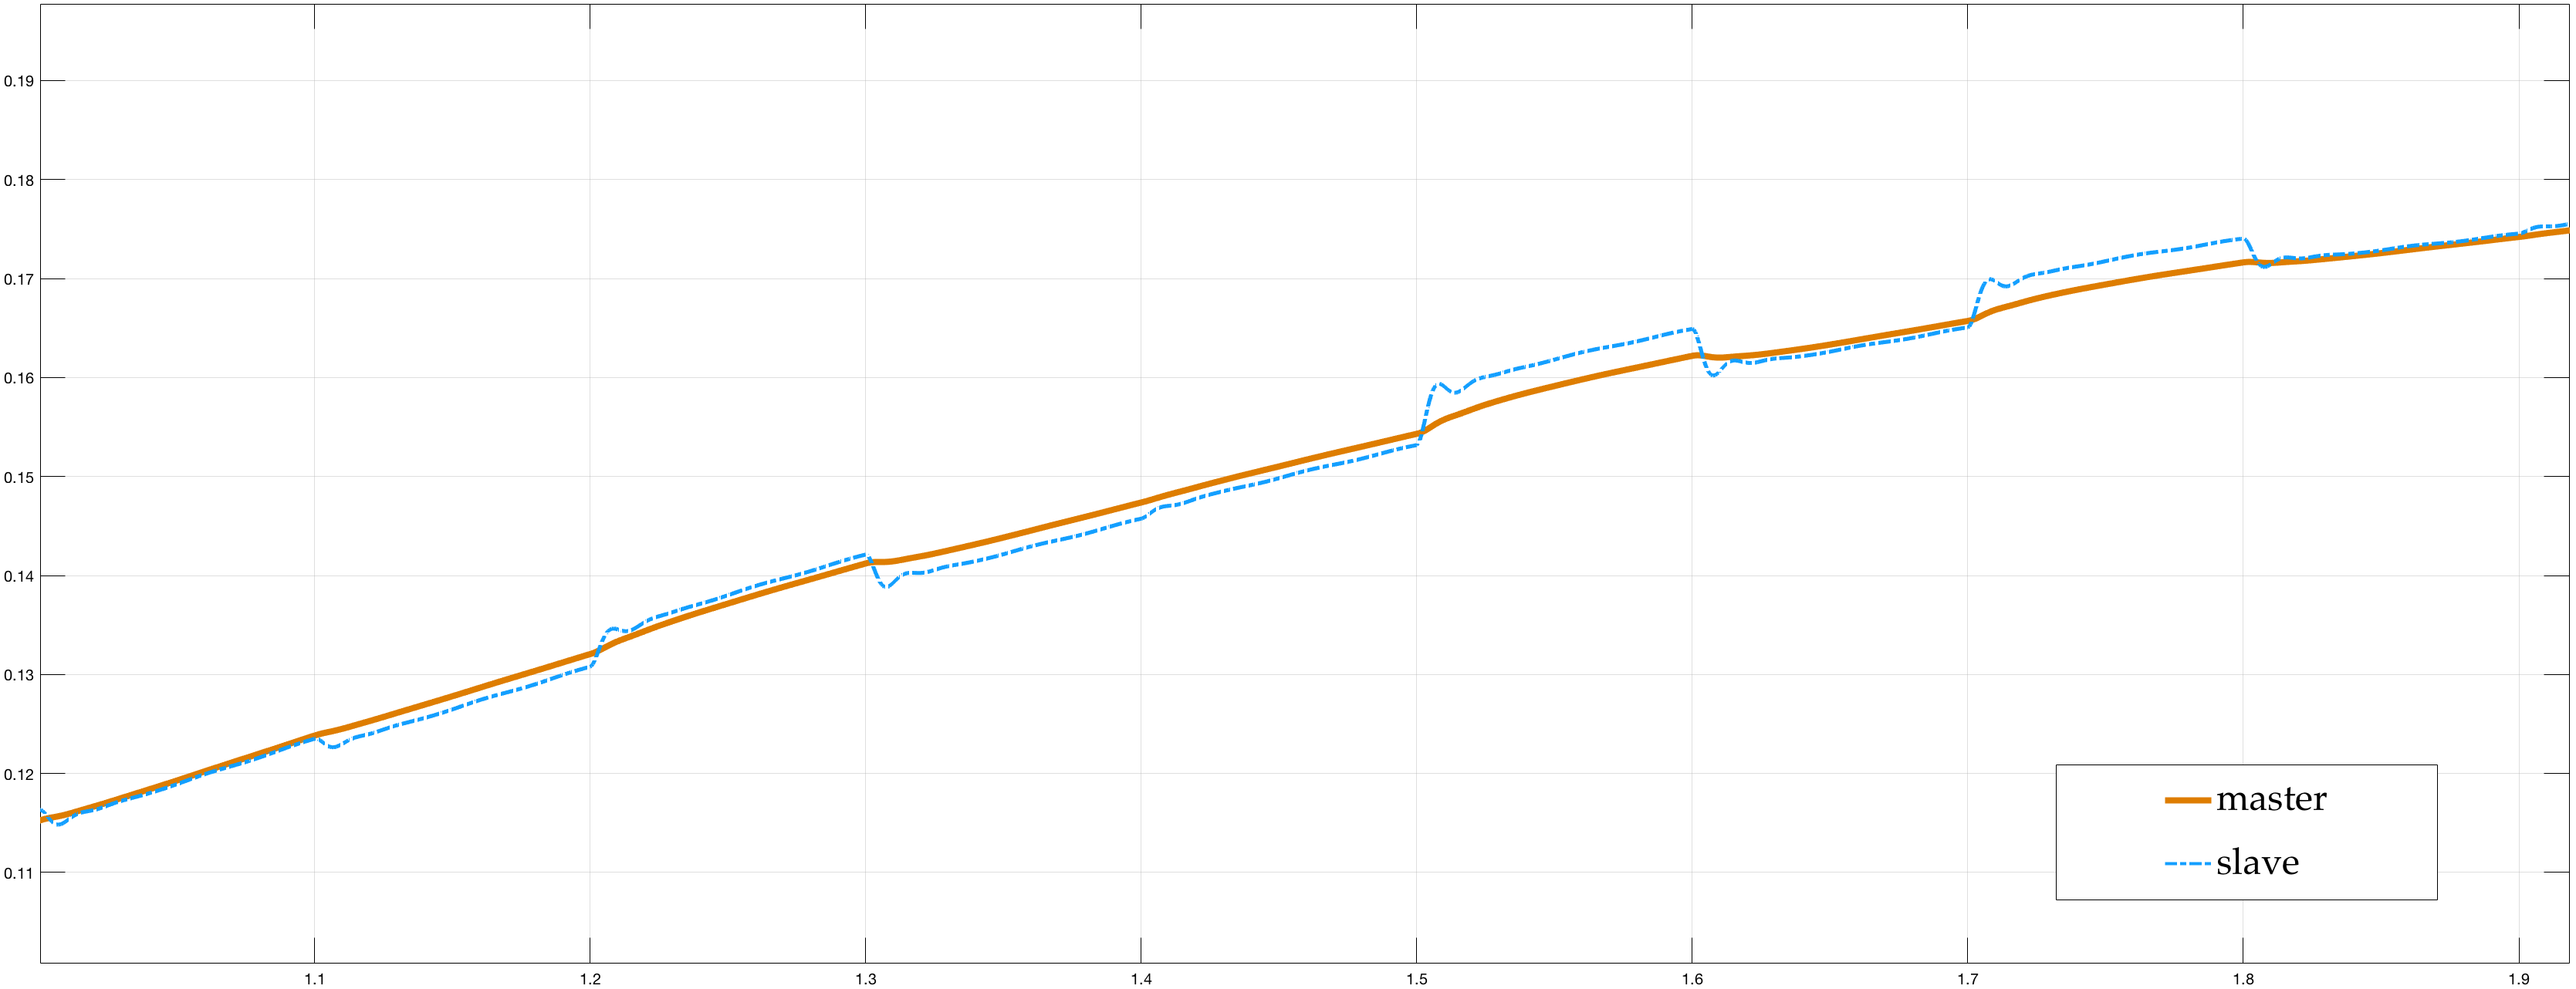
\includegraphics[width=\textwidth,
height=0.45\textwidth]{../reportTeleop/Images/freerigidPart20Htznoise}\\
\smallskip
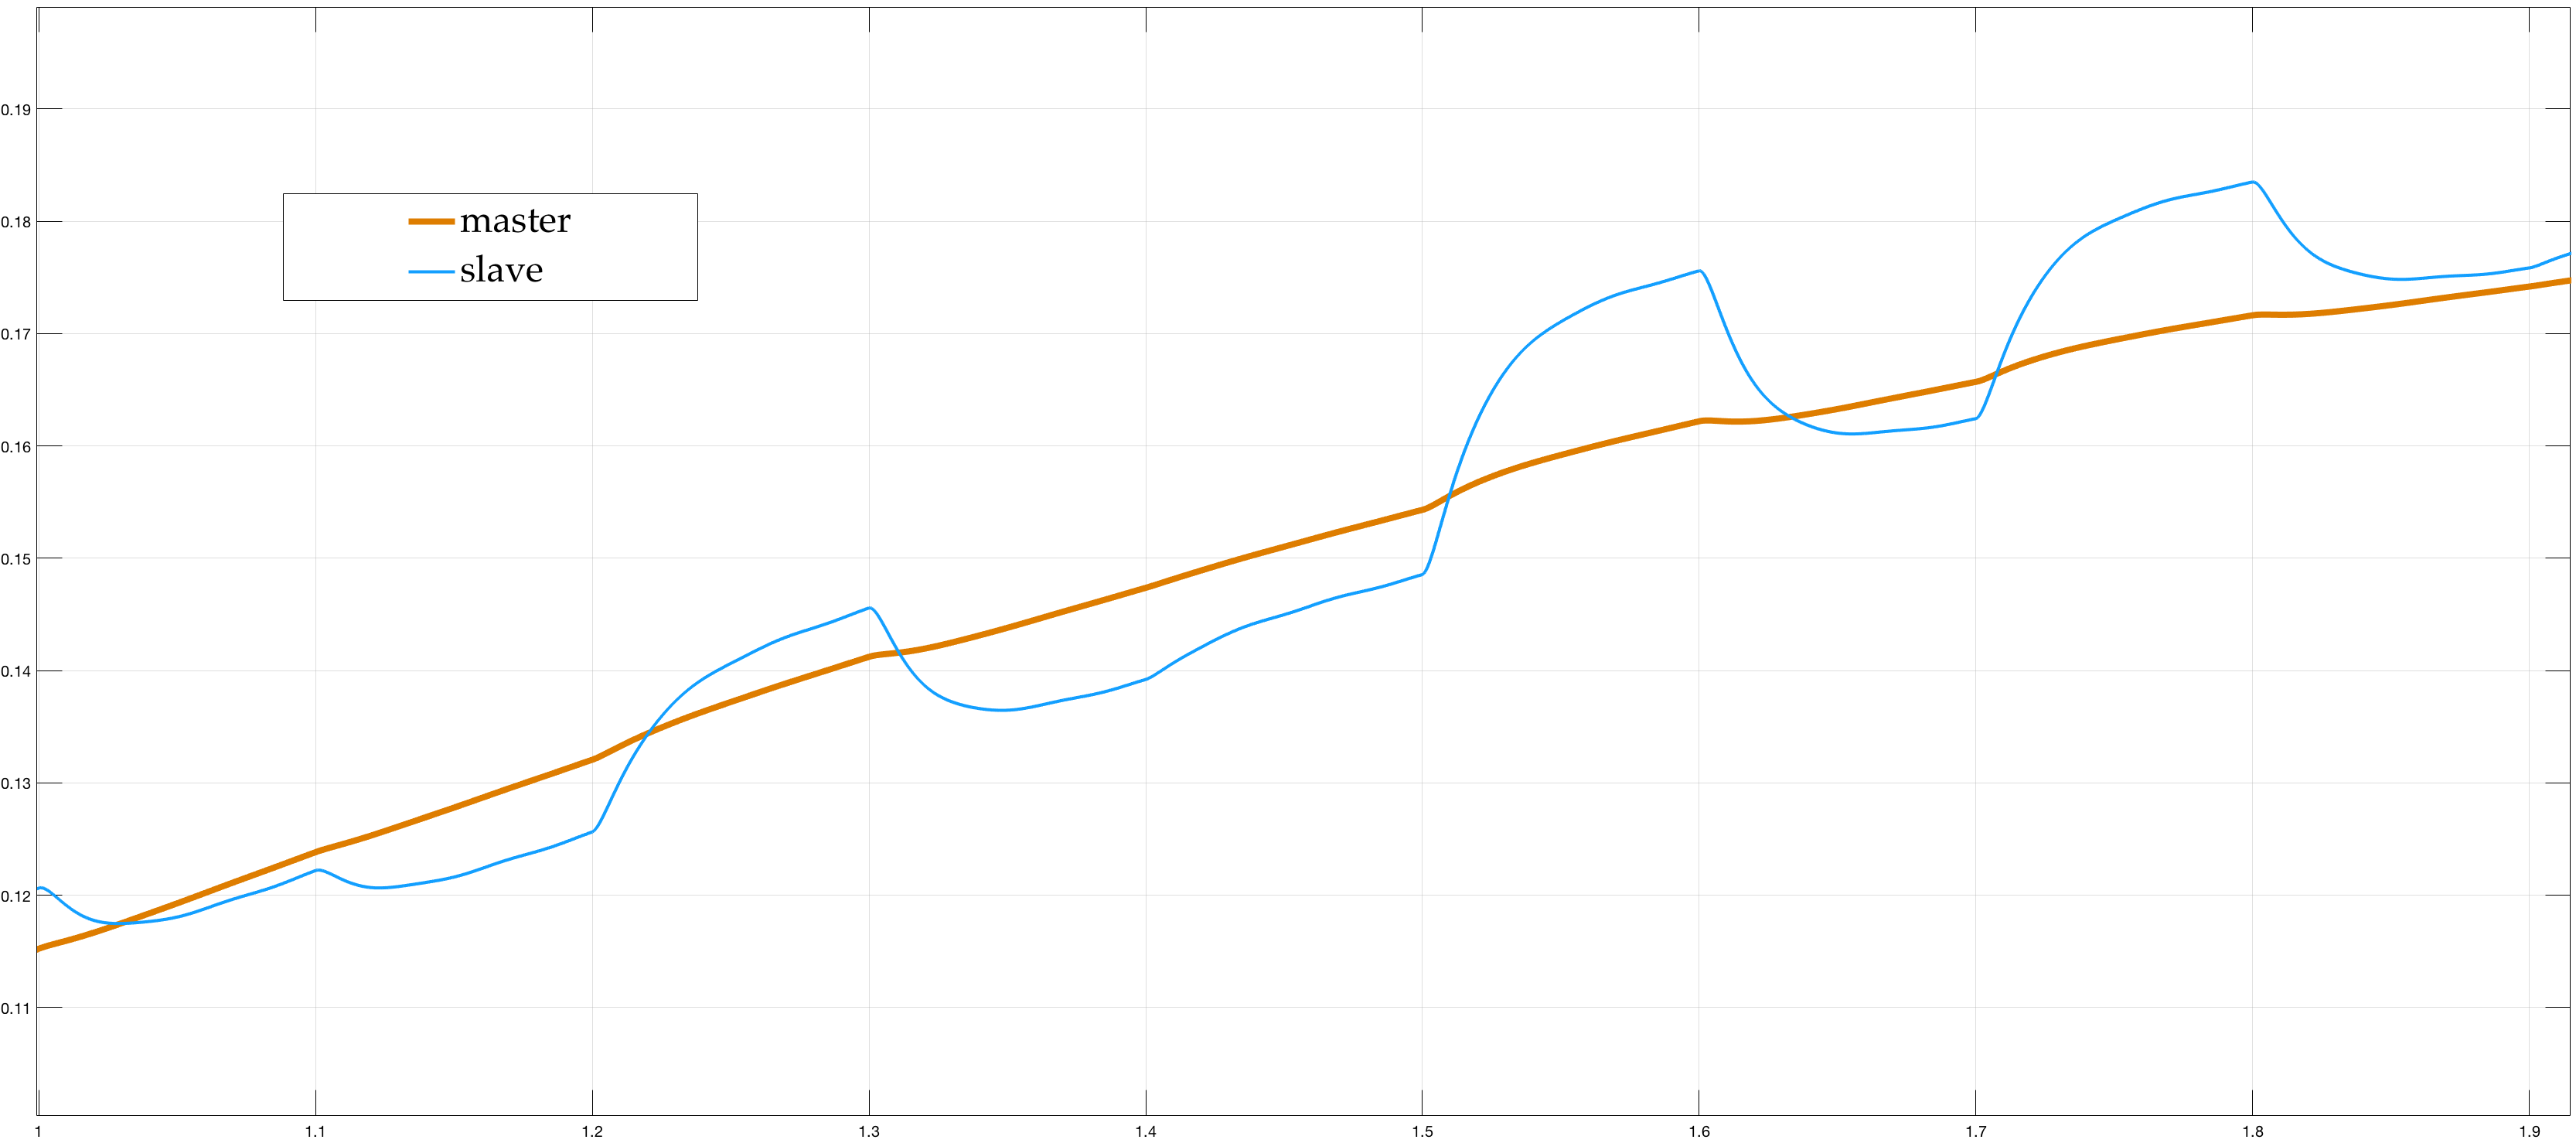
\includegraphics[width=\textwidth,
height=0.45\textwidth]{../reportTeleop/Images/freeSet20Part20Htznoise}
\end{columns}
\end{frame}

\begin{frame}{Task execution: In contact}
  \smallskip
  \begin{columns}
    \column{.20\textwidth}
    \color{Orange}\textbf{Rigid coupling:}\\
    lower error \\
    \bigskip
    \bigskip
    \bigskip
    \color{black}\textbf{Position tracking error }\\
    \bigskip
    \bigskip
    \bigskip
    \color{LightBlue}\textbf{Virtual compliance:}\\
    higher error

    \column{.85\textwidth}
    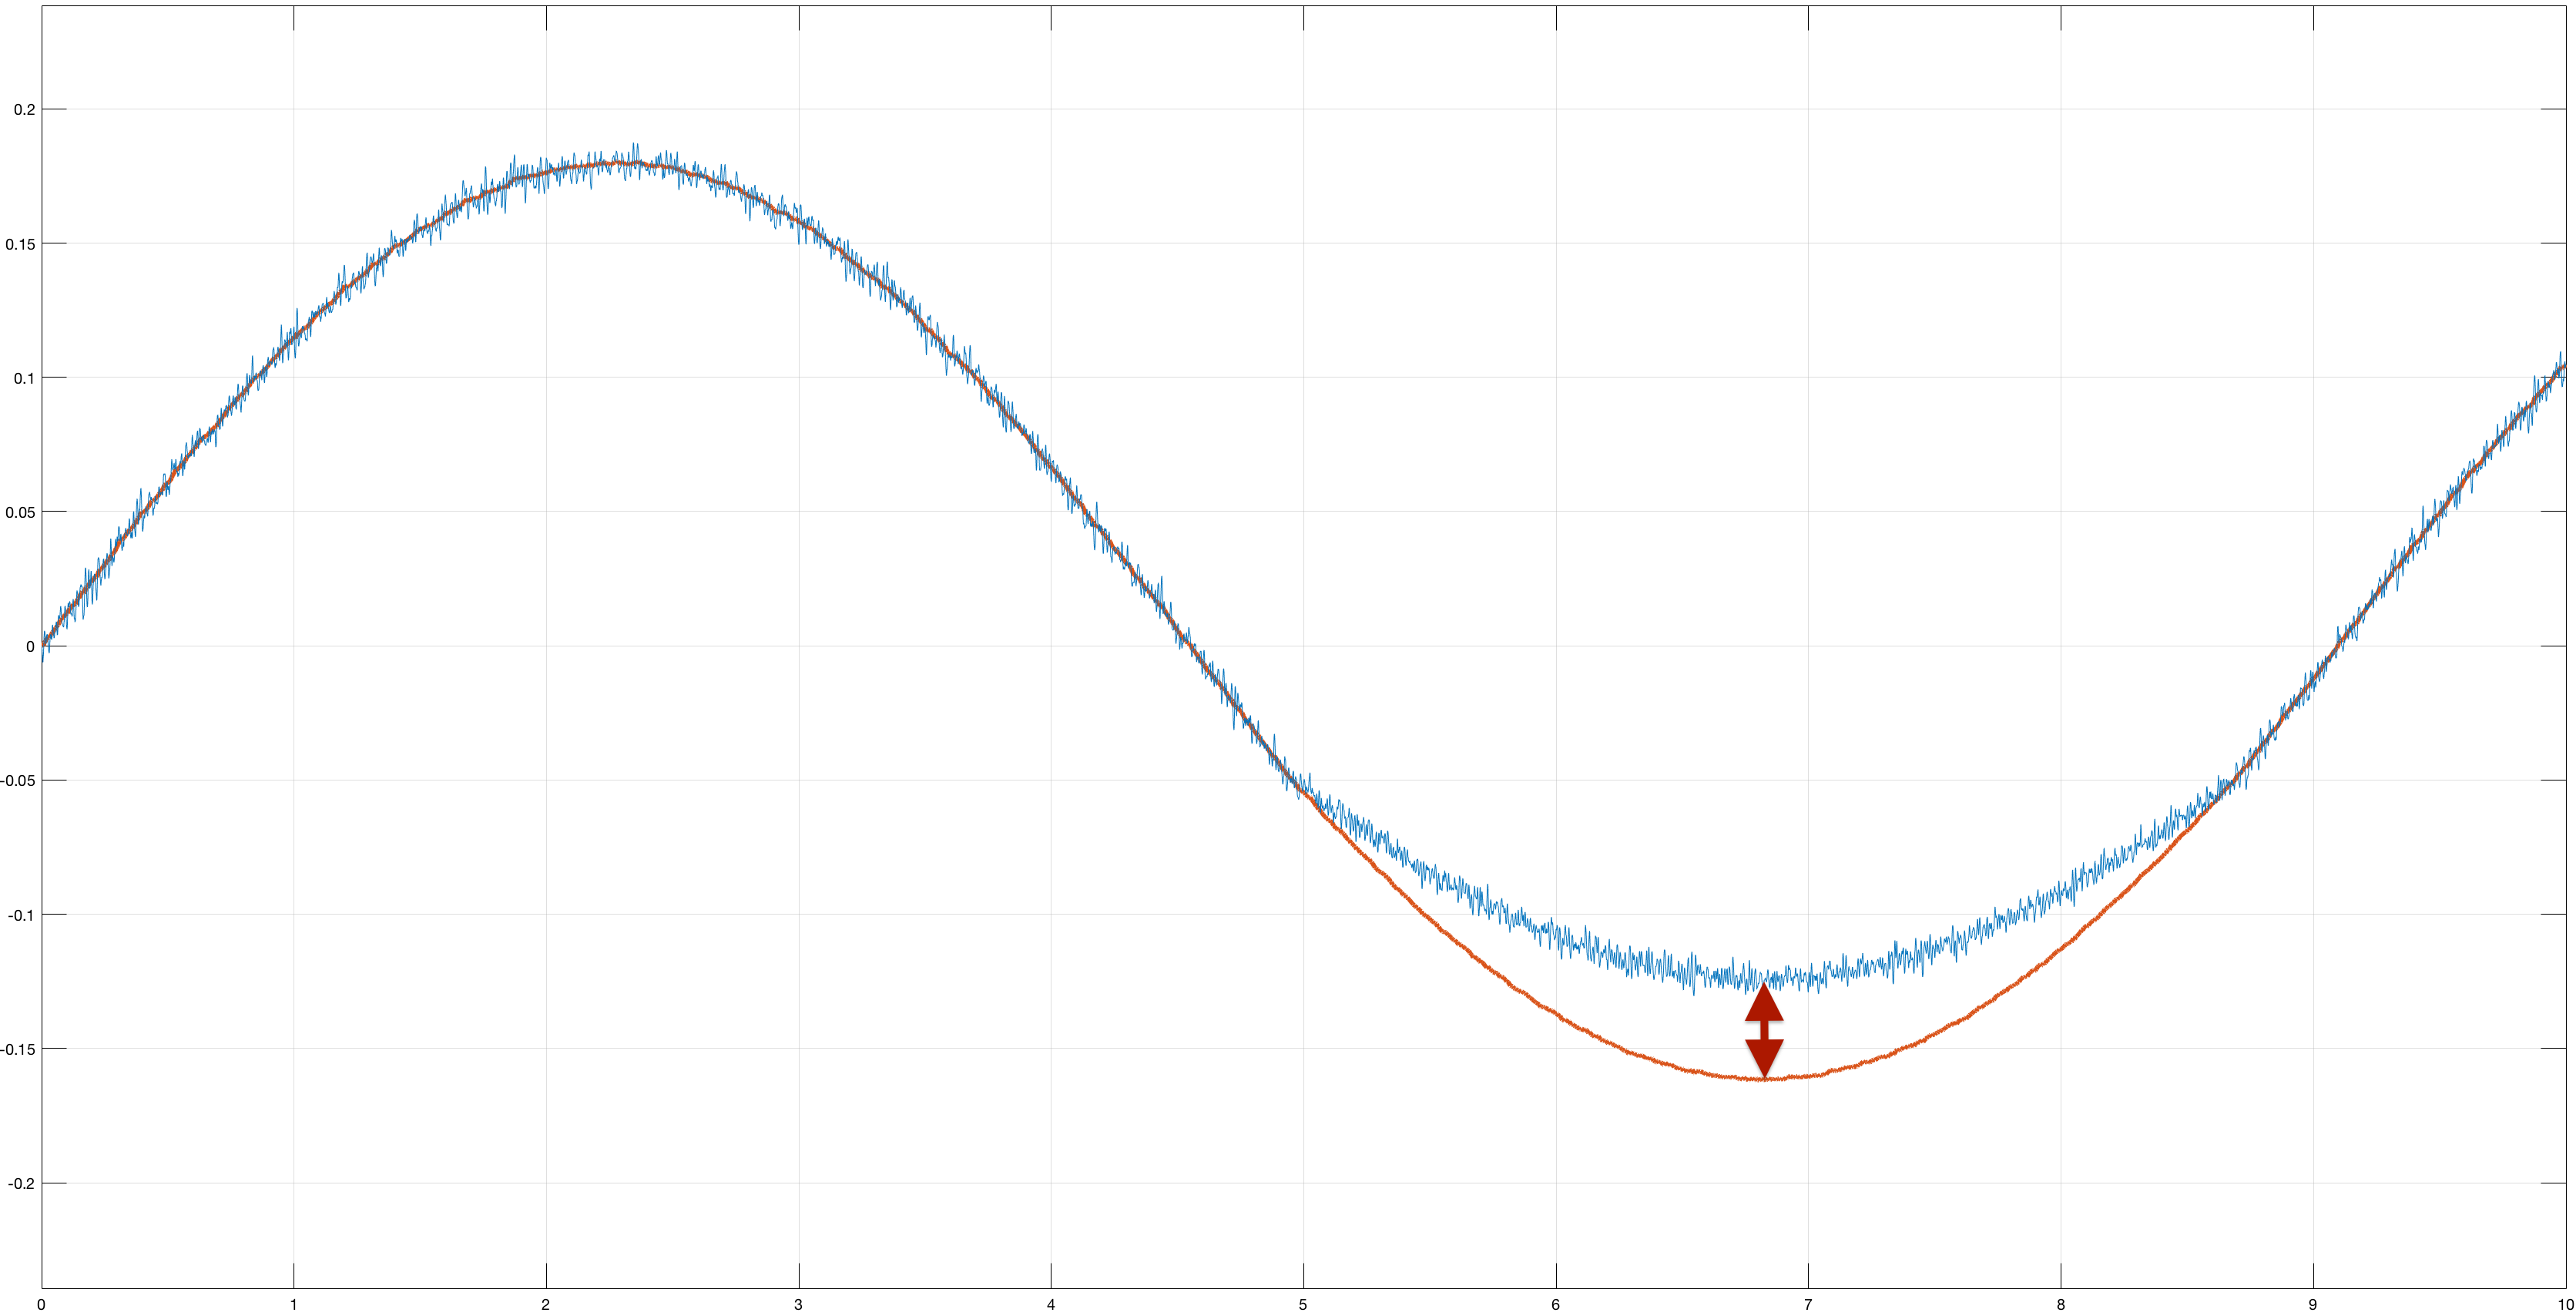
\includegraphics[width=\textwidth,
    height=0.43\textwidth]{../reportTeleop/Images/rigidContactReacPosArrow}
    \smallskip
    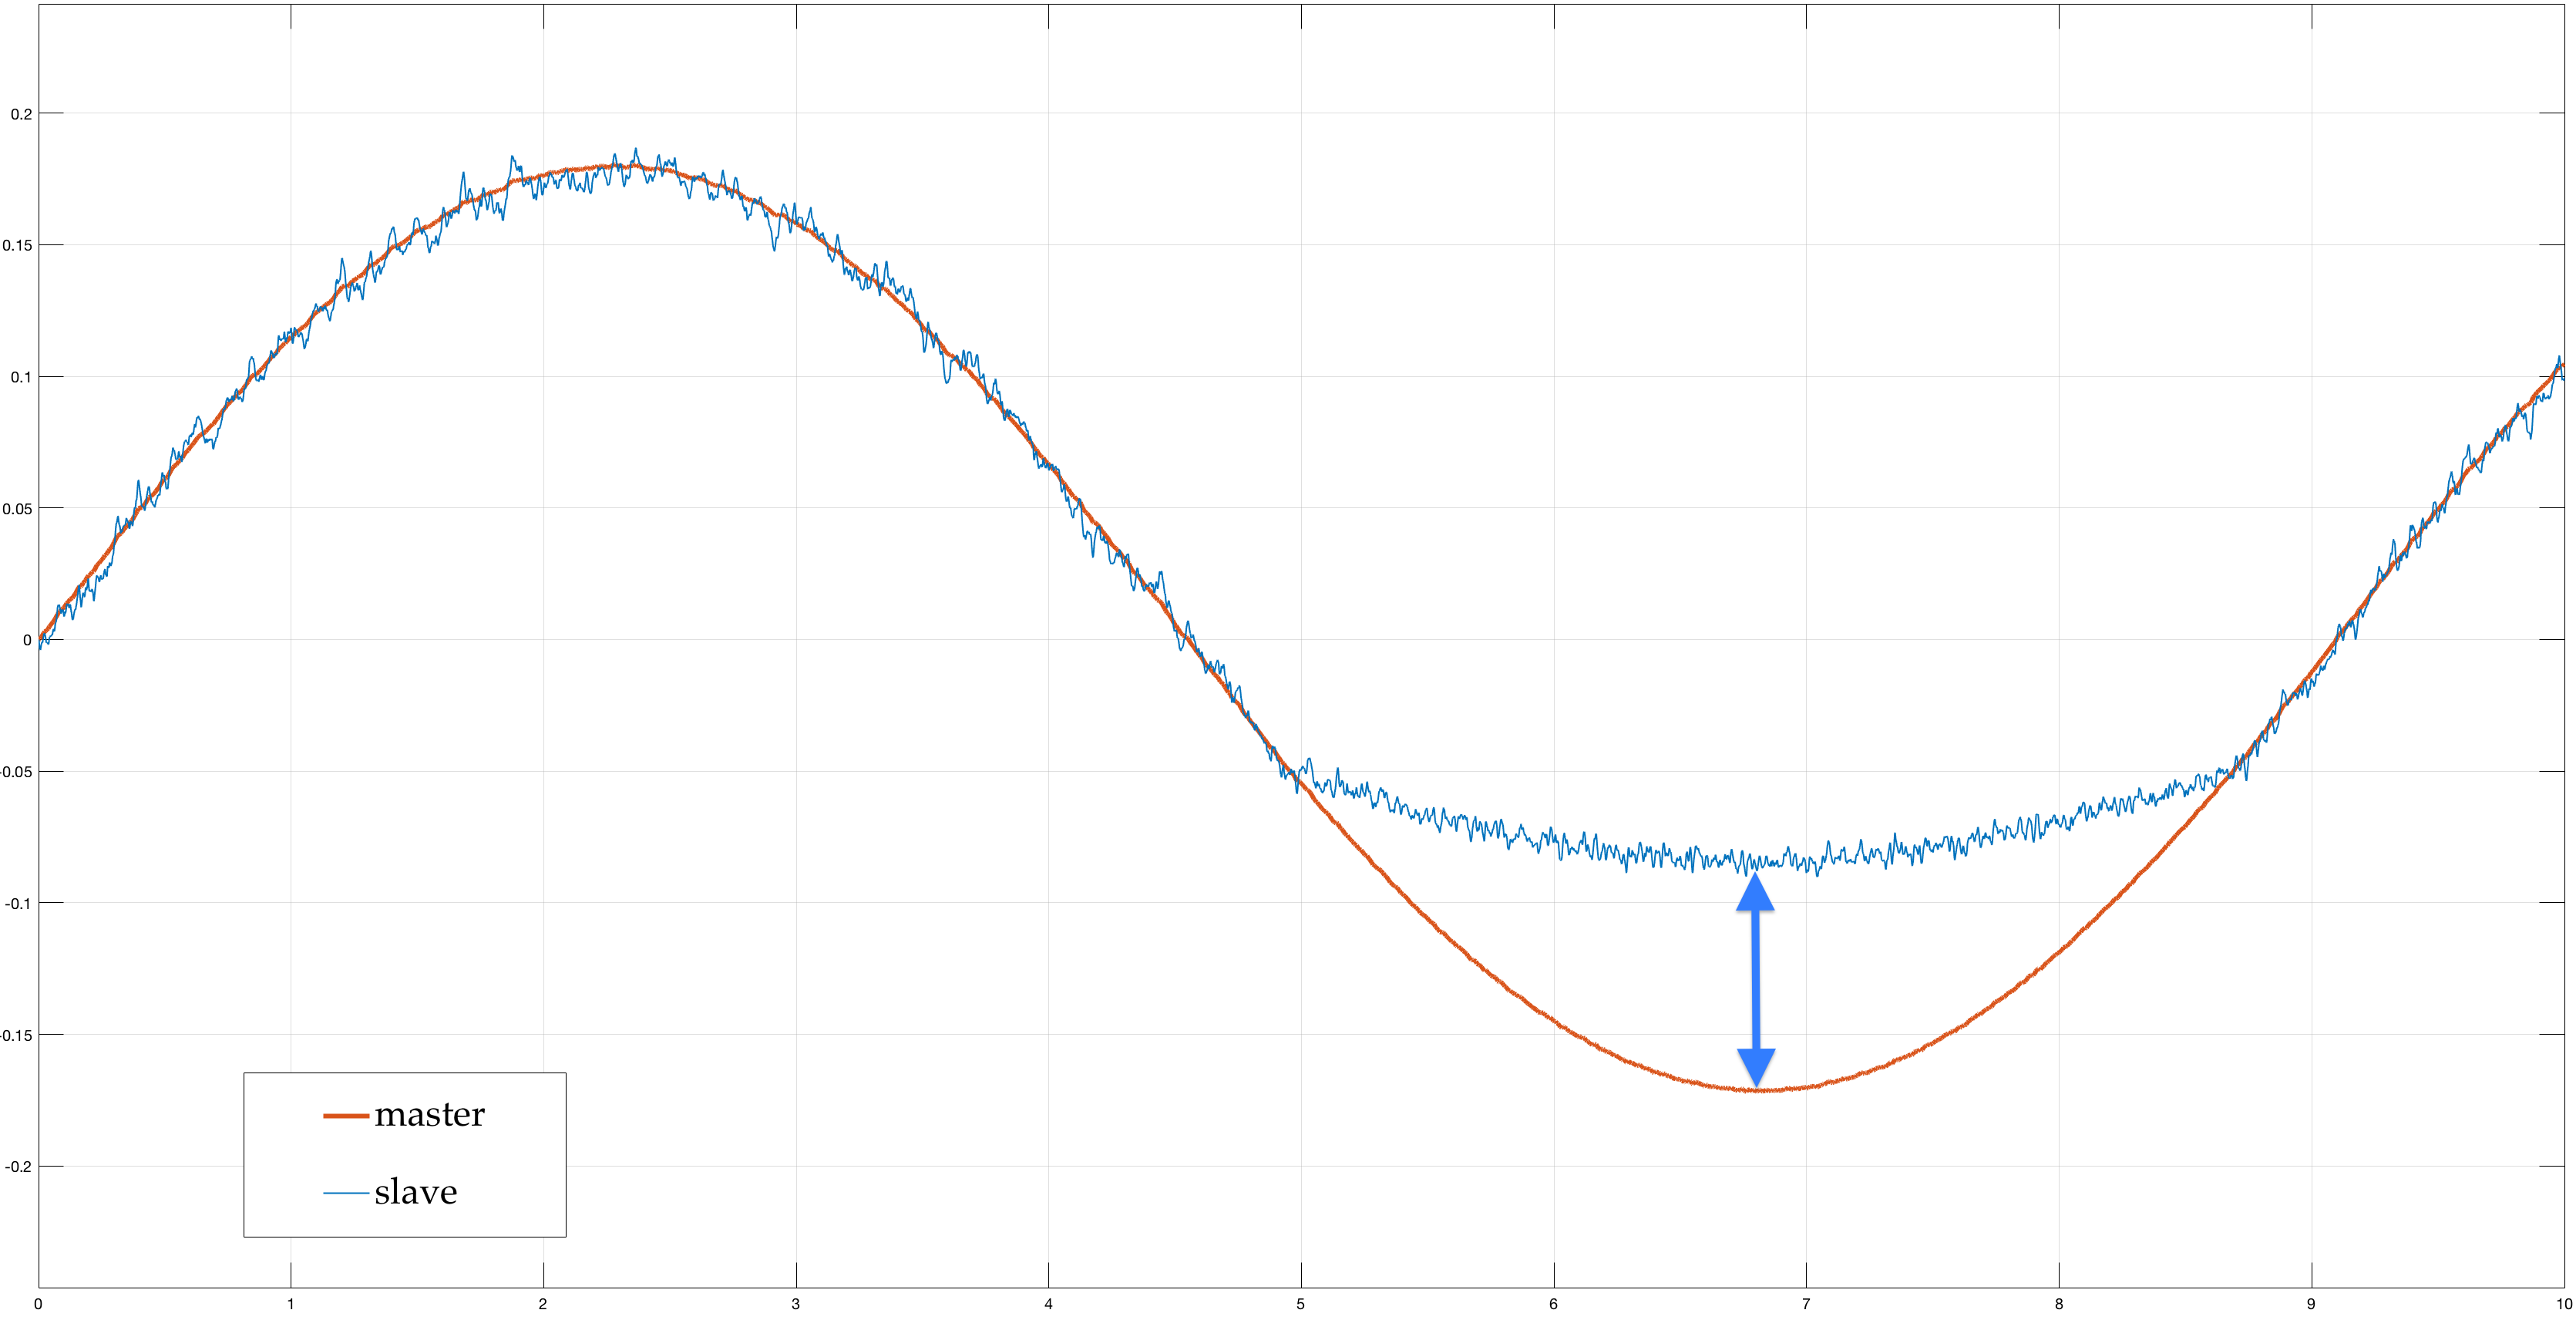
\includegraphics[width=\textwidth,
    height=0.43\textwidth]{../reportTeleop/Images/setPointContactReacPosArrow}\\

 \end{columns}
\end{frame}

\begin{frame}{Task execution: In contact}
  \smallskip
  \begin{columns}
    \column{.20\textwidth}
    \color{Orange}\textbf{Rigid coupling:}\\
    higher torque noise\\
    \bigskip
    \bigskip
    \bigskip
    \color{LightBlue}\textbf{Virtual compliance:}\\
    lower torque noise
    \column{.85\textwidth}
    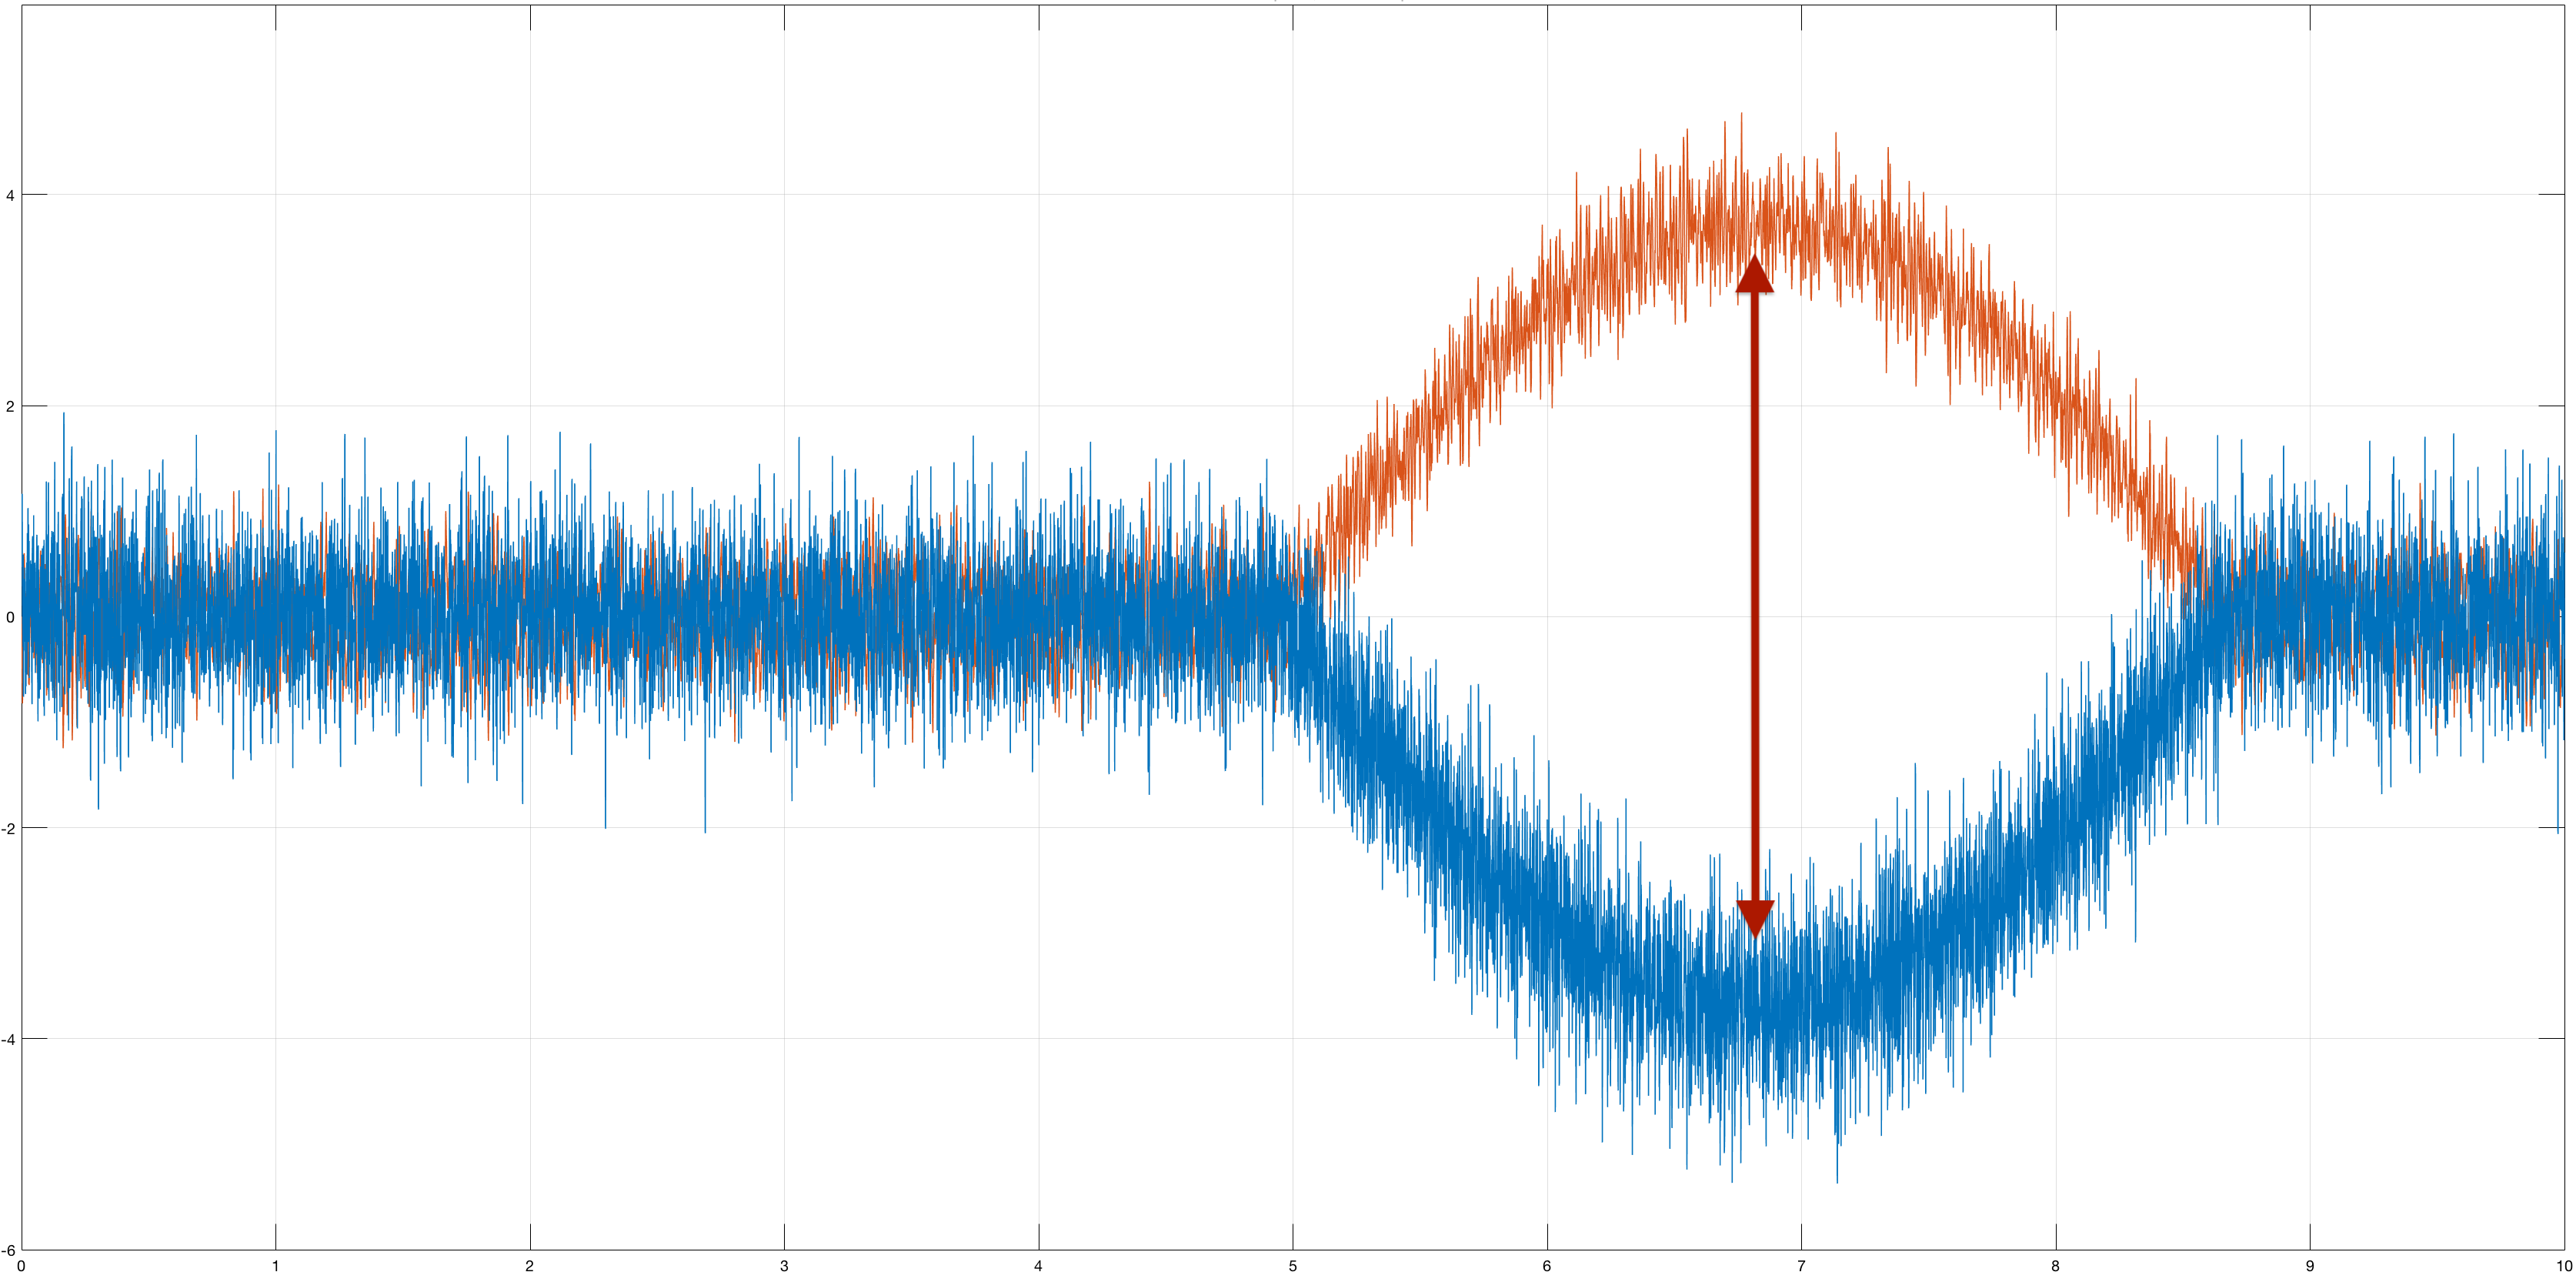
\includegraphics[width=\textwidth,
    height=0.43\textwidth]{../reportTeleop/Images/rigidContactReacTorArrow}
    \smallskip
    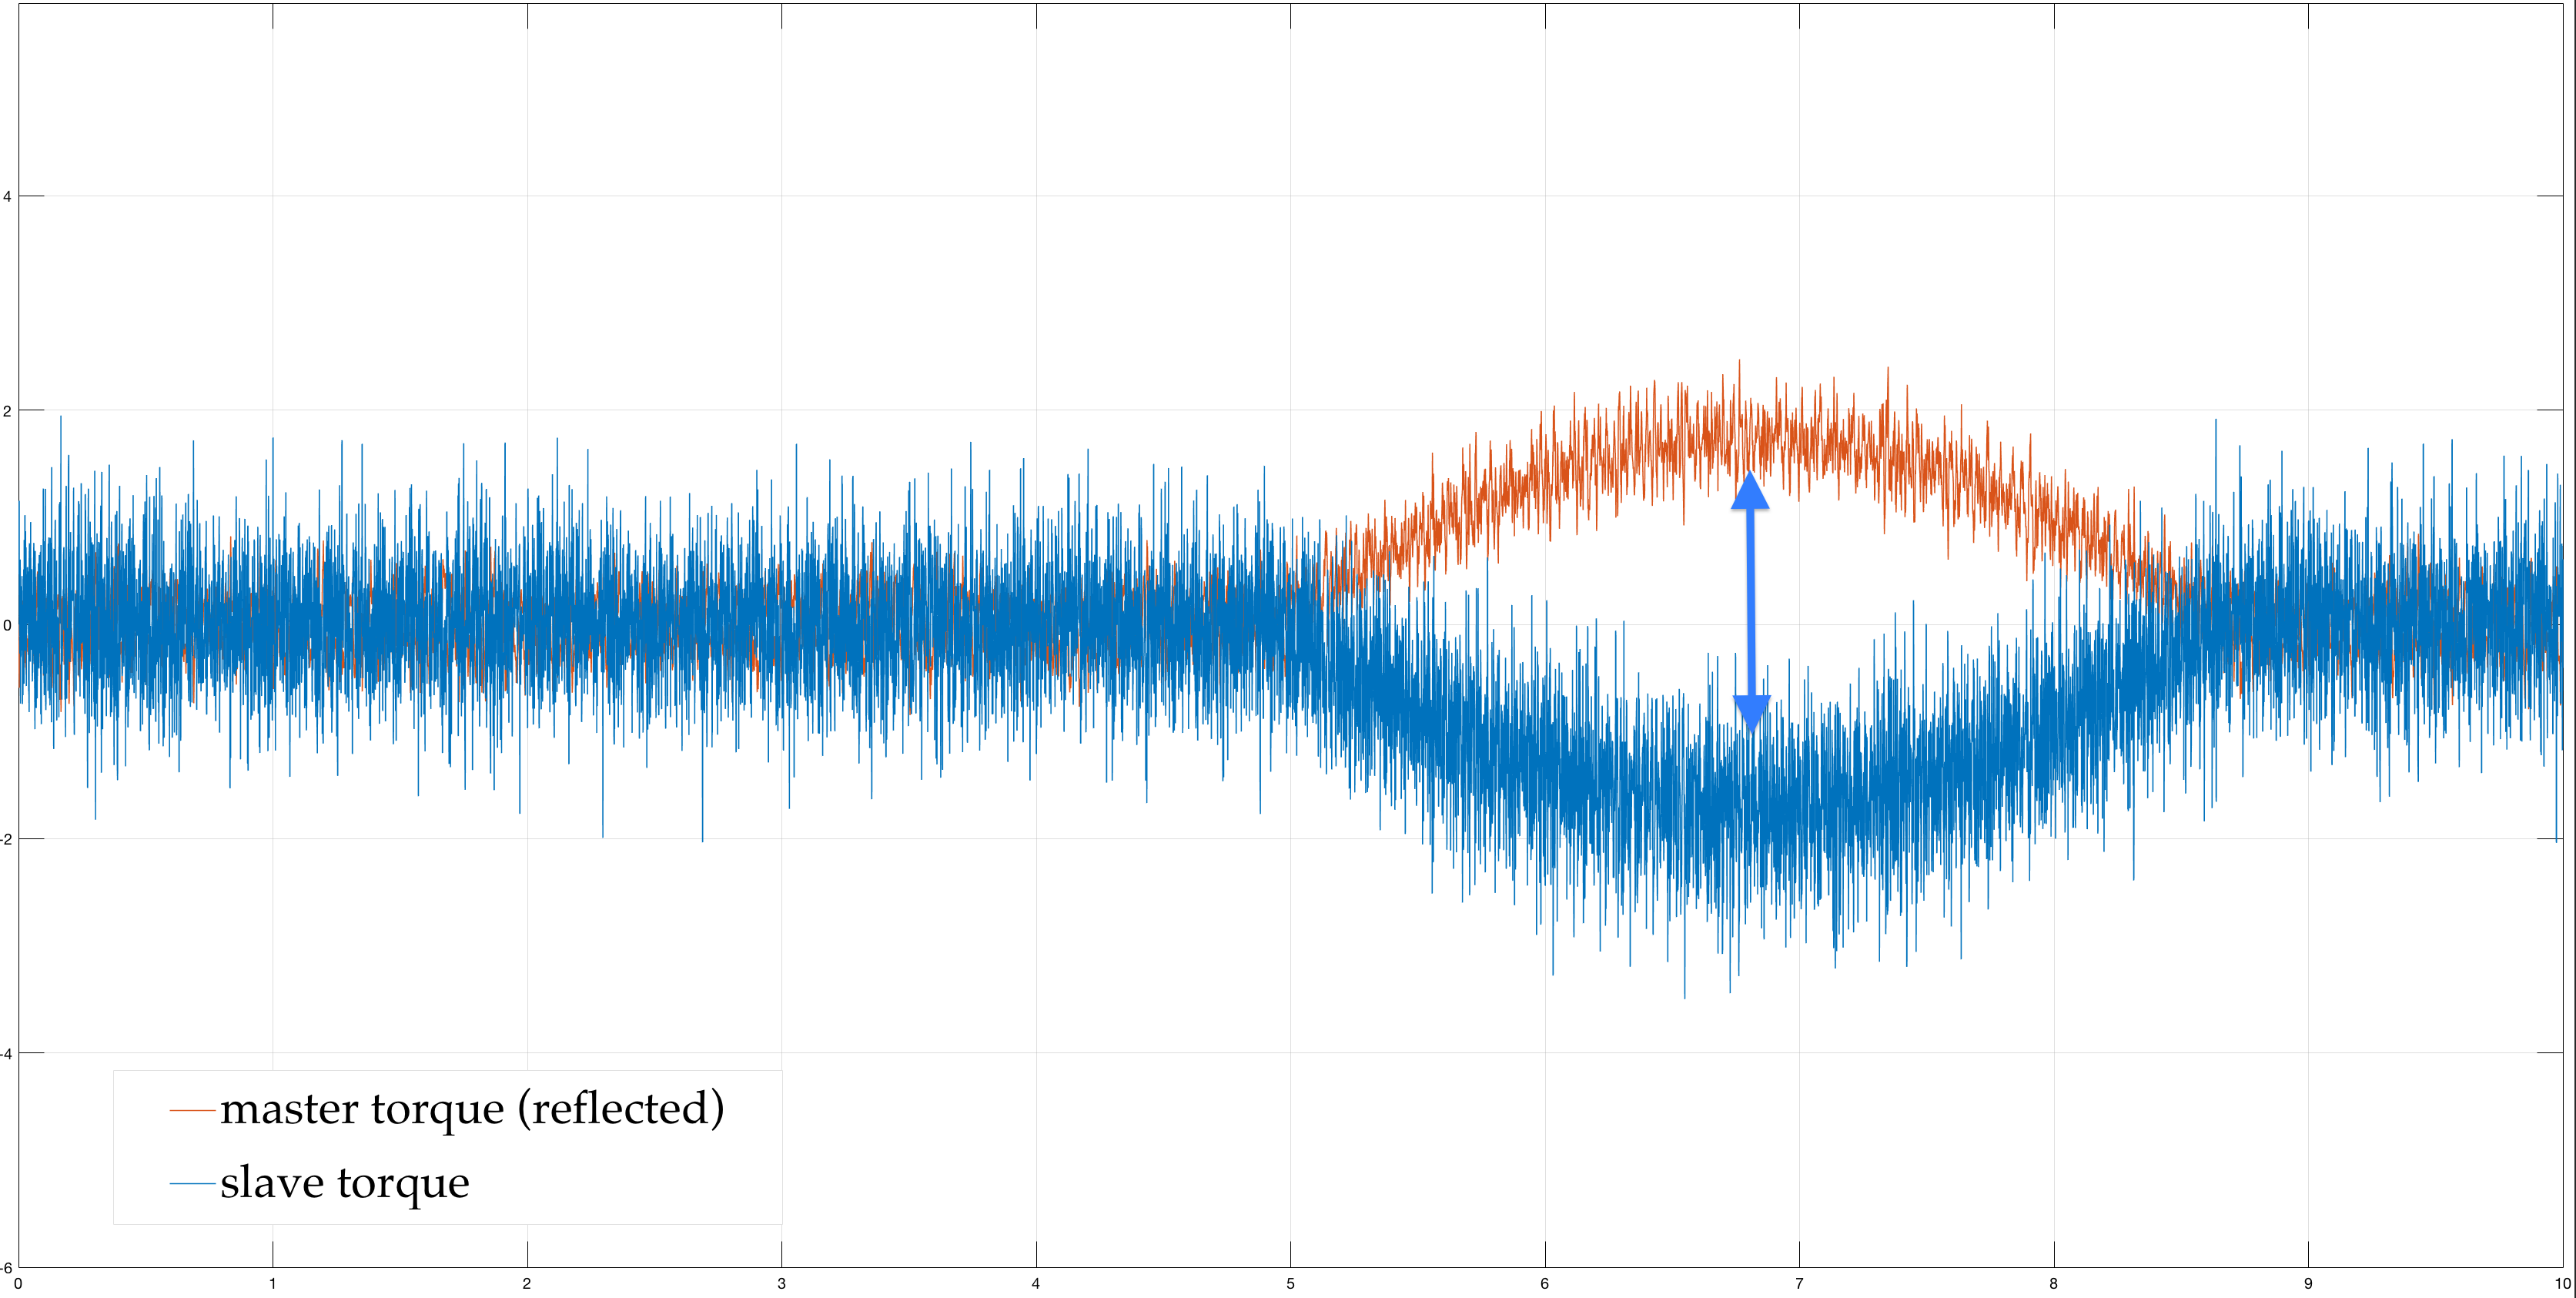
\includegraphics[width=\textwidth,
    height=0.43\textwidth]{../reportTeleop/Images/setPointContactReacTorArrow}\\

 \end{columns}
\end{frame}


\begin{frame}{Task execution: In contact}
  \color{LightBlue} Virtual compliance :
 \begin{center}
   \movie[height = 0.6\textwidth, width = 0.72\textwidth]{}{./virtualComplK20.mov}
 \end{center}
\end{frame}

\begin{frame}{Task execution: In contact}
  \color{Orange} Rigid coupling:
 \begin{center}
   \movie[height = 0.6\textwidth, width = 0.72\textwidth]{}{./rigidCoupling.mov}
 \end{center}
\end{frame}



\section{Conclusions}

\begin{frame}{Conclusions}

  \textbf{Proposed solution:} 
  \begin{itemize}
  \item based on \textbf{virtual} spring-dumper system with additional inertia;
  \item desired \textbf{cut-off} frequencies obtained regulating the \textbf{virtual} spring stiffness.
  \end{itemize}

  \textbf{Consequences:} 
  \begin{itemize}
  \item the proposed controller preserves the useful (\textsl{low}) frequency inputs and reject the noisy ones (\textsl{high}). 
%    It shows a \textbf{trade-off} between control effort and tracking error in
%    task execution.
  \item In contact motion it leads to a position gap between master and slave. It can be used only in \textbf{soft material handling} tasks.
%    Rejects high frequency signals, namely \textbf{noise} and preserves low frequency ones like \textbf{control inputs}.
  \end{itemize}
\end{frame}

{\definecolor{BlueTOL}{HTML}{222255}
\setbeamercolor{palette primary}{fg=black, bg=white}
\begin{frame}[standout]
Thank you for your attention!
\end{frame}
}

\appendix



\end{document}
